\documentclass{scrreprt}
\usepackage{listings}
\usepackage{underscore}
\usepackage{graphicx}
\usepackage[bookmarks=true]{hyperref}
\usepackage[utf8]{inputenc}
\usepackage[croatian]{babel}
\usepackage{fancyhdr}
\usepackage{lastpage}
\fancyhf{}
\rfoot{Stranica \thepage \hspace{1pt} od \pageref{LastPage}}
\hypersetup{
    bookmarks=false,
    pdftitle={Software Requirement Specification},
    pdfauthor={Petar Matišić},
    pdfsubject={TeX and LaTeX},
    pdfkeywords={TeX, LaTeX, graphics, images},
    colorlinks=true, % false: boxed links; true: colored links
    linkcolor=blue,
    citecolor=black,
    filecolor=black,
    urlcolor=purple,
    linktoc=page
}%
\def\myversion{1.0 }
\date{}
%\title
\usepackage{hyperref}
\begin{document}

\begin{flushright}
    \rule{16cm}{5pt}\vskip1cm
    \begin{bfseries}
        \Huge{SPECIFIKACIJA\\ SOFTVERSKIH ZAHTJEVA}\\
        \vspace{1cm}
        za\\
        \vspace{1cm}
         e-dnevnik o specijalističkom usavršavanju doktora medicine\\
        \vspace{1cm}
        \LARGE{Verzija \myversion}\\
        \vspace{1cm}
        \begin{itemize}
        \item Autori:
        \item[] Petar Matišić,
        \item[] Dorian Badel,
        \item[] Mihael Kožul,
        \item[] Tomislava Cafuk\\
        \item Mentor: dr.sc. Marko Mijač
        \end{itemize}
        \vspace{1.8cm}
    \end{bfseries}
\end{flushright}
\begin{center} \large{Programsko inženjerstvo}, \today \end{center}
\thispagestyle{empty}

\tableofcontents
\thispagestyle{empty}

\chapter{UVOD}

\setcounter{page}{3}
\section{Svrha}
Ovaj dokument predstavlja specifikaciju softverskih zahtjeva za softver namijenjen evidentiranju o specijalističkom usavršavanju doktora medicine uz pomoć dnevnika rada. Specifikacija zahtjeva je izrađena na temelju inicijalnih korisničkih zahtjeva dostavljenih od strane Povjerenstva za mlade liječnike Hrvatske liječničke komore. Ciljana skupina specifikacije zahtjeva su: $specijalizant$, koji obavlja privatnu praksu kao doktor medicine kojem je na temelju prijedloga tijela, odnosno osoba iz članka 8. Pravilnika o spec. usavršavanju izdano rješenje ministra o odobrenju specijalizacije, zatim $glavni$ $mentor$, koji je odgovoran za propisano provođenje cjelokupnog programa specijalističkog usavršavanja, te $mentor$, koji je odgovoran za točnost podataka u dnevniku rada doktora medicine na specijalističkom usavršavanju. Osim kao podloga za daljnji razvoj softverskog rješenja, ovaj dokument ima i svrhu ugovora između naručitelja (Ministarstvo zdravstva i Ministarstvo znanosti i obrazovanja) i izvođača (Hrvatske liječničke komore) pa ciljana skupina čitatelja uključuje i naručitelje.\\
Sama struktura dokumenta se temelji na predlošku definiranom u dokumentu $IEEE$ $830-1998$ $Recommended$ $Practice$ $for$ $Software$ $Requirements$ $Specifications$.

\section{Opseg}
Specijalizant ima obavezu svakodnevno voditi evidenciju rada na specijalizaciji u Knjižici o specijalističkom usavršavanju doktora medicine i u Dnevniku rada doktora medicine na specijalističkom usavršavanju. Ovo rješenje se odnosi na Dnevnik rada. Vođenje evidencija u fizičkoj knjižici je nepraktično zbog raznih redundancija. Potreba fizičkog kontakta s mentorom i glavnim mentorom kako bi odobrili i evaluirali rad specijalizanta je suvišna. e-Dnevnik za specijalističko usavršavanje dnevnika medicine (dalje e-Dnevnik) će se koristiti tijekom rada specijalizanta. Sve što se inače popunjavalo u Dnevnik rada pretvorit će se u digitalni oblik s novim sučeljem. Jednostavniji unos podataka s automatskim popunjavanjem polja poput današnjeg datuma i sl. Mentor i glavni mentor će u svakom trenu imati uvid u podatke unesene sa strane specijalizanta i moći će ga vrednovati od bilo gdje sa samo par klikova. Softversko rješenje ubrzat će proces bilježenja u dnevnik rada i osloboditi više vremena za stjecanje novih vještina.

\section{Definicije, akronimi i skraćenice}
$Specijalizacija$ jest oblik organiziranog stjecanja kompetencija prema propisanom programu koja se
može obavljati samo u ovlaštenim zdravstvenim ustanovama, trgovačkim društvima koja obavljaju
zdravstvenu djelatnost, odnosno kod ovlaštenih doktora medicine koji obavljaju privatnu praksu, a koji
ispunjavaju uvjete propisane člankom 4 ili 5 Pravilnika.\\
$Program$ $specijalizacije$ definira sadržaj i trajanje svih dijelova specijalističkog usavršavanja, popis
općih i posebnih kompetencija, uvjete koje moraju ispunjavati pravne i fizičke osobe za obavljanje
specijalističkog usavršavanja, obrazac praćenja napredovanja u stjecanju kompetencija, obrazac
praćenja obavljenih zahvata, a uključuje i poslijediplomski specijalistički studij za grane specijalizacije
kada je to Pravilnikom propisano.\\
$Ishodi$ $u$č$enja$ obuhvaćaju iskaz o tome što specijalizant treba naučiti, razumjeti ili biti sposoban učiniti
nakon završenog programa specijalizacije.\\
$Specijalizant$ jest doktor medicine kojem je ministar nadležan za zdravstvo (u daljnjem tekstu: ministar)
izdao rješenje o odobrenju specijalizacije i s kojim je zdravstvena ustanova čiji je osnivač Republika
Hrvatska, jedinica područne (regionalne) samouprave ili grad zasnovala radni odnos na neodređeno
vrijeme s probnim radom od šest mjeseci. Radni odnos specijalizant može zasnovati i u drugoj
zdravstvenoj ustanovi, trgovačkom društvu koje obavlja zdravstvenu djelatnost ili kod zdravstvenog
radnika privatne prakse. Specijalizant jest i doktor medicine koji obavlja privatnu praksu te doktor
medicine kojem je na temelju prijedloga tijela, odnosno osoba iz članka 8 ovog Pravilnika izdano
rješenje ministra o odobrenju specijalizacije.\\
$Glavni$ $mentor$ jest doktor medicine specijalist sa znanstveno-nastavnim ili stručnim zvanjem iste
specijalističke grane za koju se specijalizant usavršava ili doktor medicine specijalist iste specijalističke
grane za koju se specijalizant usavršava, s najmanje deset godina specijalističkog staža. Glavnog mentora imenuje ministar rješenjem o odobrenju specijalizacije. Glavni mentor može biti mentor istovremeno za najviše pet specijalizanata. Glavni mentor je odgovoran za propisano provođenje cjelokupnog programa specijalističkog usavršavanja.\\
$Mentor$ jest doktor medicine specijalist iste specijalističke grane za koju se specijalizant usavršava s
najmanje pet godina specijalističkog staža. Mentora imenuje ministar rješenjem o odobrenju specijalizacije.\\
\textbf{MZ} – Ministarstvo zdravstva\\
\textbf{MZO} – Ministarstvo znanosti i obrazovanja\\
\textbf{HLK} – Hrvatska liječnička komora

\section{Reference}
\begin{enumerate}
    \item “830-1998 - IEEE Recommended Practice for Software Requirements Specifications.” IEEE, 1998. [Online]. Available: http://ieeexplore.ieee.org/servlet/opac?punumber=5841
    \item Dokumenti opisa problemske domene.
\end{enumerate}

\section{Struktura dokumenta}
\textbf{U poglavlju $2$ – Općeniti opis} e-Dnevnik je stavljen u kontekst sustava te se opisuje interakcija kako s korisnicima, tako i s drugim sustavima, softverskim rješenjima, hardverom, i komunikacijskim tehnologijama. Zatim se opisuju osnovne funkcije koje će e-Dnevnik izvršavati te tip korisnika koji će ga koristiti. Osim toga prikazana su i ograničenja koja mogu utjecati na sam razvoj softverskog rješenja.\\
\textbf{U poglavlju $3$ – Funkcionalni zahtjevi} se definiraju funkcionalni zahtjevi za razvoj e-Dnevnika na onoj razini detalja koja je dovoljna dizajnerima i programerima da započnu sa osmišljavanjem i implementacijom rješenja, kao i testerima da osmisle testne slučajeve.\\
\textbf{U poglavlju $4$ – Nefunkcionalni zahtjevi} se definiraju nefunkcionalni zahtjevi za razvoj e-Dnevnika koje bi dizajneri i programeri trebali uzeti u obzir prilikom osmišljavanja cjelokupnog rješenja, odnosno arhitekture, odabira implementacijskih tehnologija i pristupa.\\
\textbf{U poglavlju $5$ – Skice zaslona} vizualizirana je prvotna verzija grafičkog sučelja preko kojeg je korisnik u interakciji s e-Dnevnikom.

\chapter{OPĆENITI OPIS}

\section{Perspektiva proizvoda}
e-Dnevnik je zamišljen kao samostalno softversko rješenje koje je zamjena za postojeći sustav (temeljen na papirnatom dnevniku) za evidentiranja specijalističkog usavršavanja doktora medicine. Softversko rješenje bi trebalo sadržavati klijentsku aplikaciju koja će se izvoditi na računalu krajnjeg korisnika, dok bi baza podataka bila centralizirana zbog potrebe dijeljenja podataka između mentora. Izravna interakcija sa drugim sustavima koji nisu sastavni dio e-Dnevnika nije predviđena. S obzirom da je predviđen uvoz podataka o specijalizantima, postoji neizravna ovisnost prema dokumentima HLK.\\
e-Dnevnik nema potrebu izravnog korištenja hardverskih ili komunikacijskih tehnologija. Predviđeno je da bilo kakva uporaba takvih resursa bude odrađena od strane operacijskog sustava ili “runtime” okruženja.

\section{Funkcije proizvoda}
Budući korisnici softverskog rješenja e-Dnevnik očekuju od softvera sljedeće mogućnosti:\\
\begin{itemize}
    \item Unos podataka o programu specijalizacije
    \item Ispunjavanje evidencije dnevnika aktivnosti, prikaza slučaja bolesnika te stručnih radova
    \item Omogućavanje odobravanja unosa u dnevnik aktivnosti i prikaza slučaja bolesnika
    \item Prikaz profila s potrebnim informacijama
    \item Predavanje zahtjeva za polaganje
    \item Evidentiranje i ocjenjivanje provjera znanja
    \item Pregled hijerarhijske strukture
\end{itemize}


\section{Karakteristike korisnika}
Korisnici koji će koristiti softversko rješenje e-Dnevnik su specijalizanti, mentori i glavni mentori. S obzirom da će svi specijalizanti koristiti softver na isti način i imati istu razinu prava, možemo reći da postoji tri korisničke uloge – specijalizant, glavni mentor i obični mentor. Ipak, od svakog korisnika aplikacije će biti zatraženo da se prijavi u aplikaciju prije korištenja sa vlastitim korisničkim podacima, kako bismo mogli razlikovati koje bilješke je evidentirao svaki od korisnika. Svi korisnici aplikacije posjeduju naprednu razinu računalne i tehničke pismenosti.

\section{Ograničenja}
S obzirom da softversko rješenje e-Dnevnik podrazumijeva rad sa privatnim izvještajima specijalizanata (ostvareni rezultati tokom specijalizacije) koji su podložni GDPR odredbama, potrebno je osigurati da samo ovlaštene osobe (oba tipa mentora) imaju pristup navedenim podacima. S obzirom na problemsku domenu i karakteristike rješenja, nije uočeno postojanje dodatnih ograničenja: ne radi se o sigurnosno kritičnoj domeni; interakcija s drugim sustavima nije izravna i ne utječe u značajnoj mjeri na razvoj samog softverskog rješenja; hardverske karakteristike današnjih računala su više nego dovoljne za rad sa softverom. Od izvođača se očekuje da razvoj softverskog rješenja e-Dnevnik bude u skladu sa dobrim praksama struke, međutim, naručitelj ne postavlja specifična ograničenja s obzirom na metodološki pristup, alate i tehnologiju izrade.

\section{Pretpostavke i ovisnosti}
Ishodi učenja usavršavanja specijalizacije doktora medicine je unaprijed definiran i nije podložan promjenama u tijeku specijalizacije, stoga se ne očekuju izvanredne izmjene zahtjeva. Također, u vremenskom periodu izrade softverskog rješenja e-Dnevnik se ne očekuju takve izmjene u odabranoj tehnologiji kakve bi izazvale promjene na razini softverskih zahtjeva.

\section{Ostalo}
Nema potrebe za elaboracijom dodatnih aspekata.

\chapter{FUNKCIONALNI ZAHTJEVI}

\section{Dinamika realizacije zahtjeva (engl. Apportioning of requirements)}
U inicijalnoj verziji softvera biti će realizirani samo zahtjevi sa najvećim prioritetom. To uključuje:
\begin{itemize}
    \item[] \textbf{FZ-1} - Sustav će omogućiti pristup samo autentificiranim korisnicima.
    \item[] \textbf{FZ-3} - Sustav će omogućiti ručni unos podataka o Programu specijalizacije iz datoteke Pravilnika o specijalističkom usavršavanju doktora medicine.
    \item[] \textbf{FZ-4} - Sustav će omogućiti ispunjavanje evidencije dnevnika aktivnosti specijalizantima.
    \item[] \textbf{FZ-8} - Sustav će omogućiti evidentiranje i ocjenjivanje provjera znanja glavnim mentorima.
    \item[] \textbf{FZ-9} - Sustav će za svakog specijalizanta moći prikazati profil s osnovnim informacijama o samom specijalizantu i programu koji pohađa.
    \item[] \textbf{FZ-12} - Sustav omogučava postavljanje i ažuriranje ishoda učenja i određivanje koje kompetencije su vezane uz koju specijalizaciju\\
\end{itemize}

U narednim verzijama planirana je realizacija ostalih zahtjeva:
\begin{itemize}
    \item[] \textbf{FZ-2} - Sustav će omogućiti uvoz podataka o odobrenim specijalizantima iz datoteke izvezene iz sustava Ministarstva zdravstva Republike Hrvatske.
    \item[] \textbf{FZ-5} - Sustav će mentorima i glavnim mentorima omogućiti odobravanje unosa u dnevnik aktivnosti i prikaza slučaja bolesnika specijalizanata (ako specijalizacija to zahtjeva).
    \item[] \textbf{FZ-6} - Sustav će omogućiti ispunjavanje evidencije prikaza slučaja bolesnika specijalizantima (ako specijalizacija to zahtjeva).
    \item[] \textbf{FZ-7} - Sustav će omogućiti ispunjavanje evidencije stručnih radova specijalizantima.
    \item[] \textbf{FZ-10} - Sustav mora omogućiti specijalistu da preda zahtjev za polaganje ispita.
    \item[] \textbf{FZ-11} - Sustav omogućava pregled svih mentora za koje je zadužen glavni mentor.
\end{itemize}

\begin{figure}[h!]
    \centering
    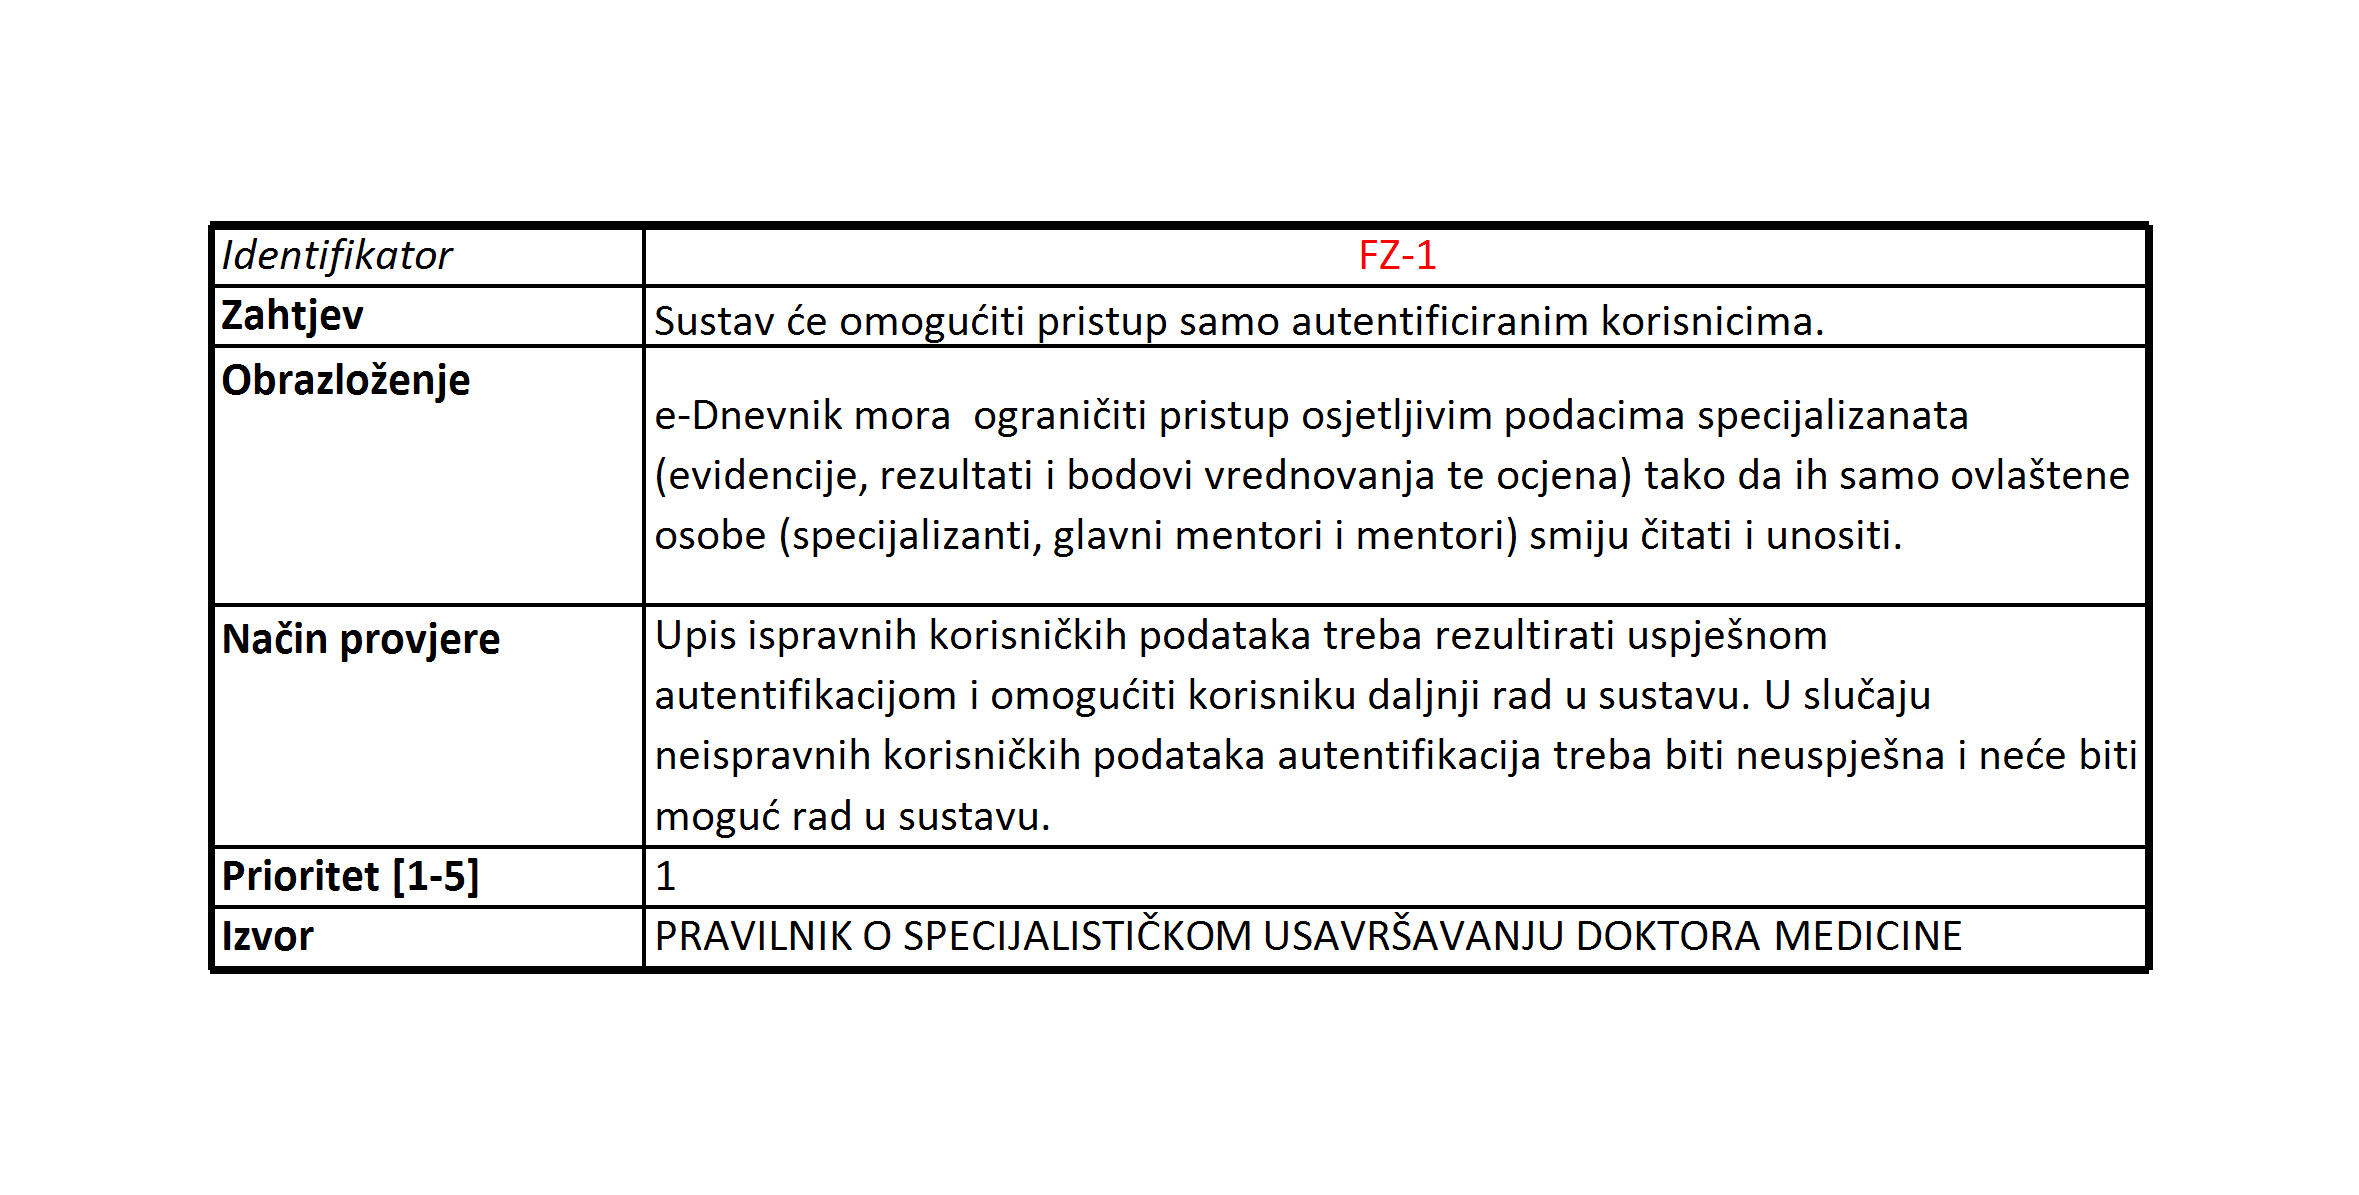
\includegraphics[width=1\textwidth]{slike/1.png}
\end{figure}
\begin{figure}[h!]
    \centering
    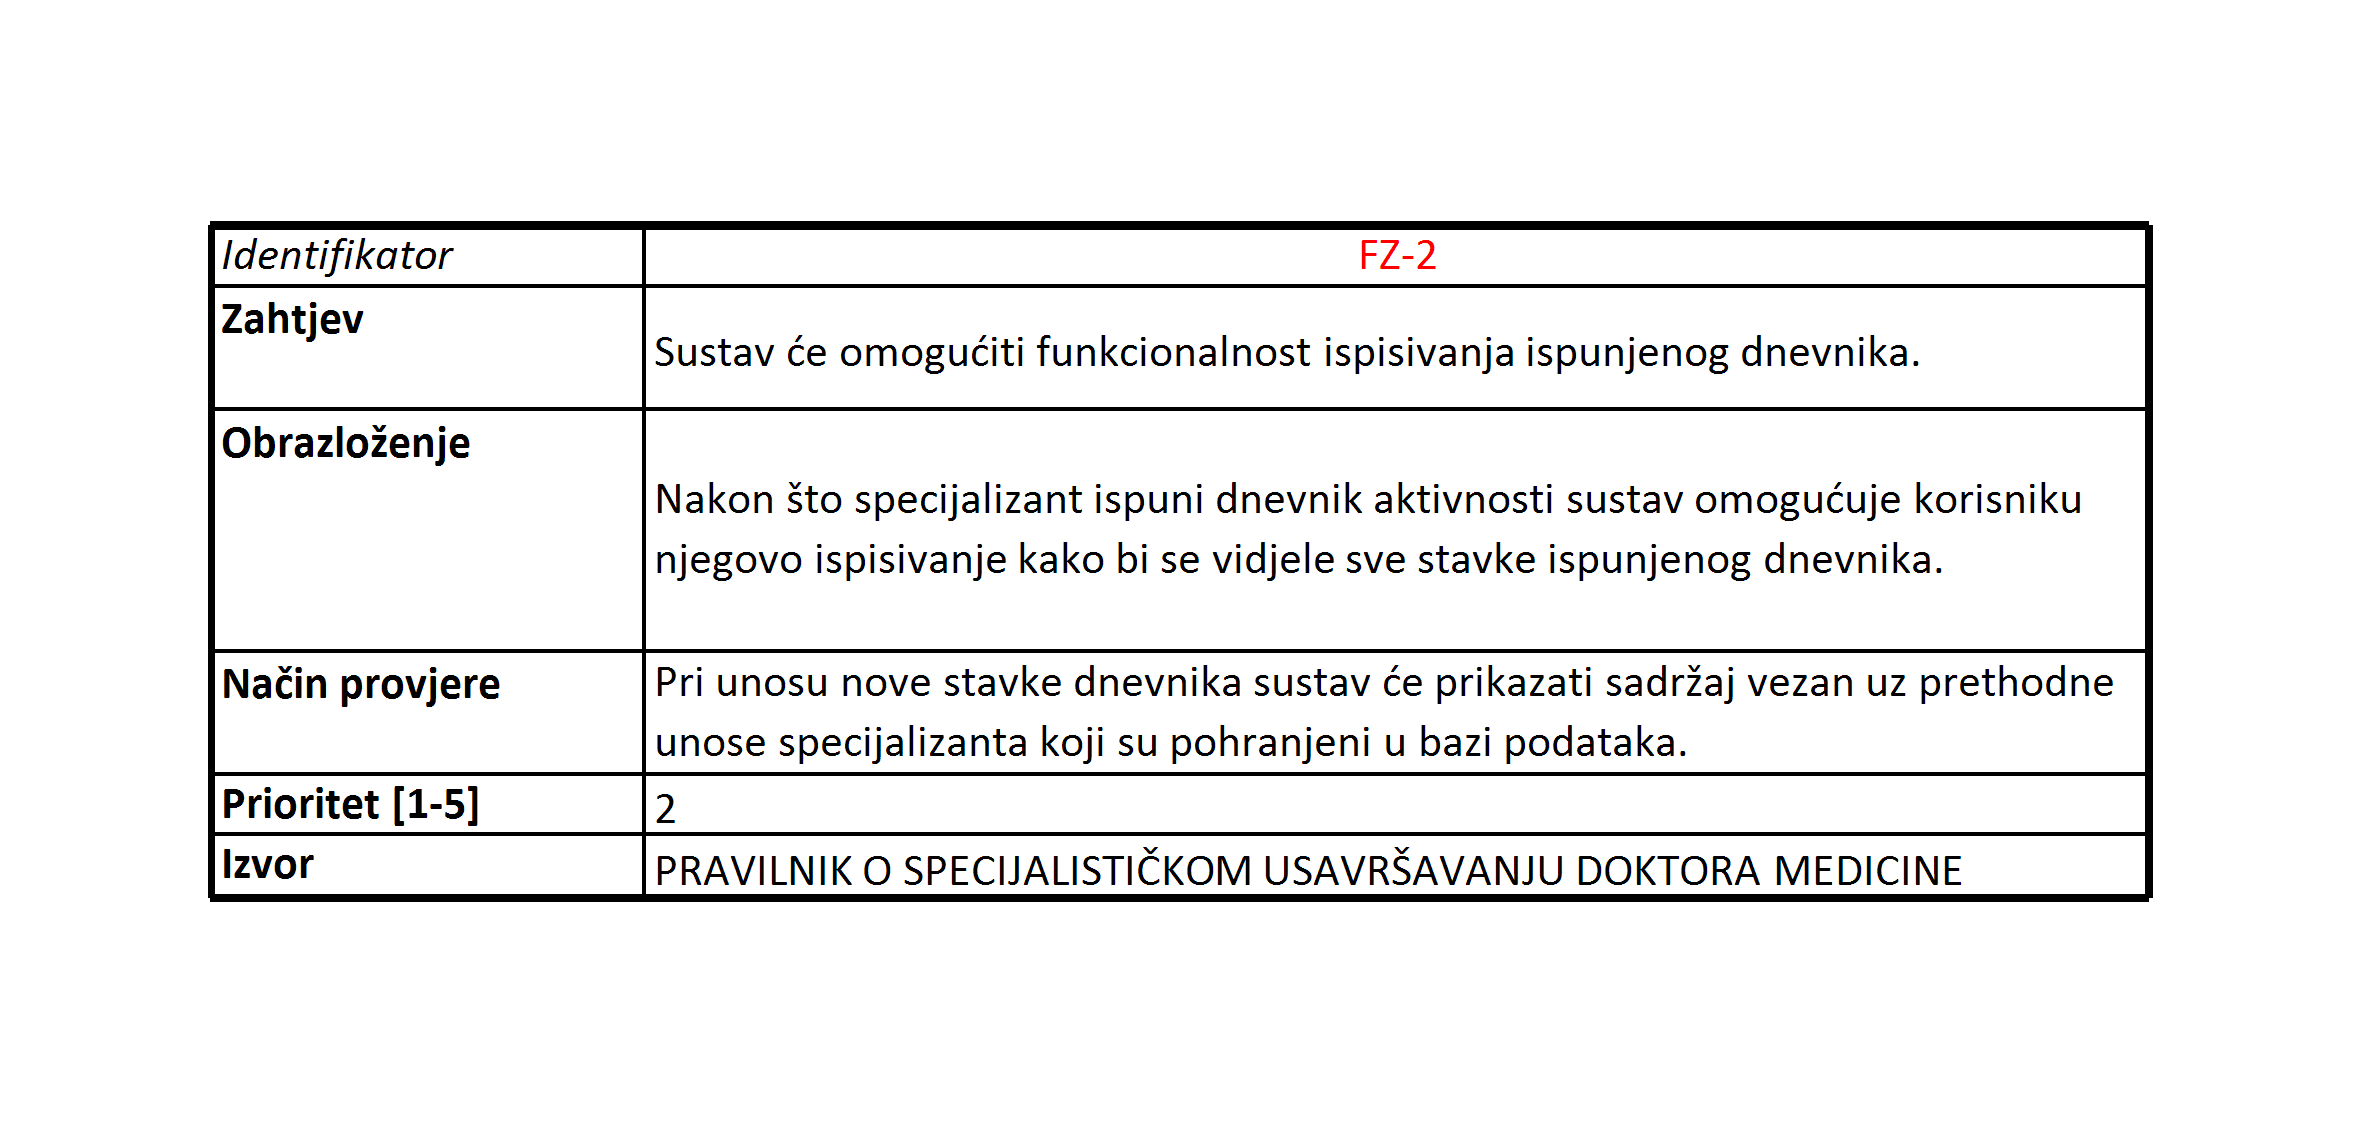
\includegraphics[width=1\textwidth]{slike/2.png}
\end{figure}
\begin{figure}[h!]
    \centering
    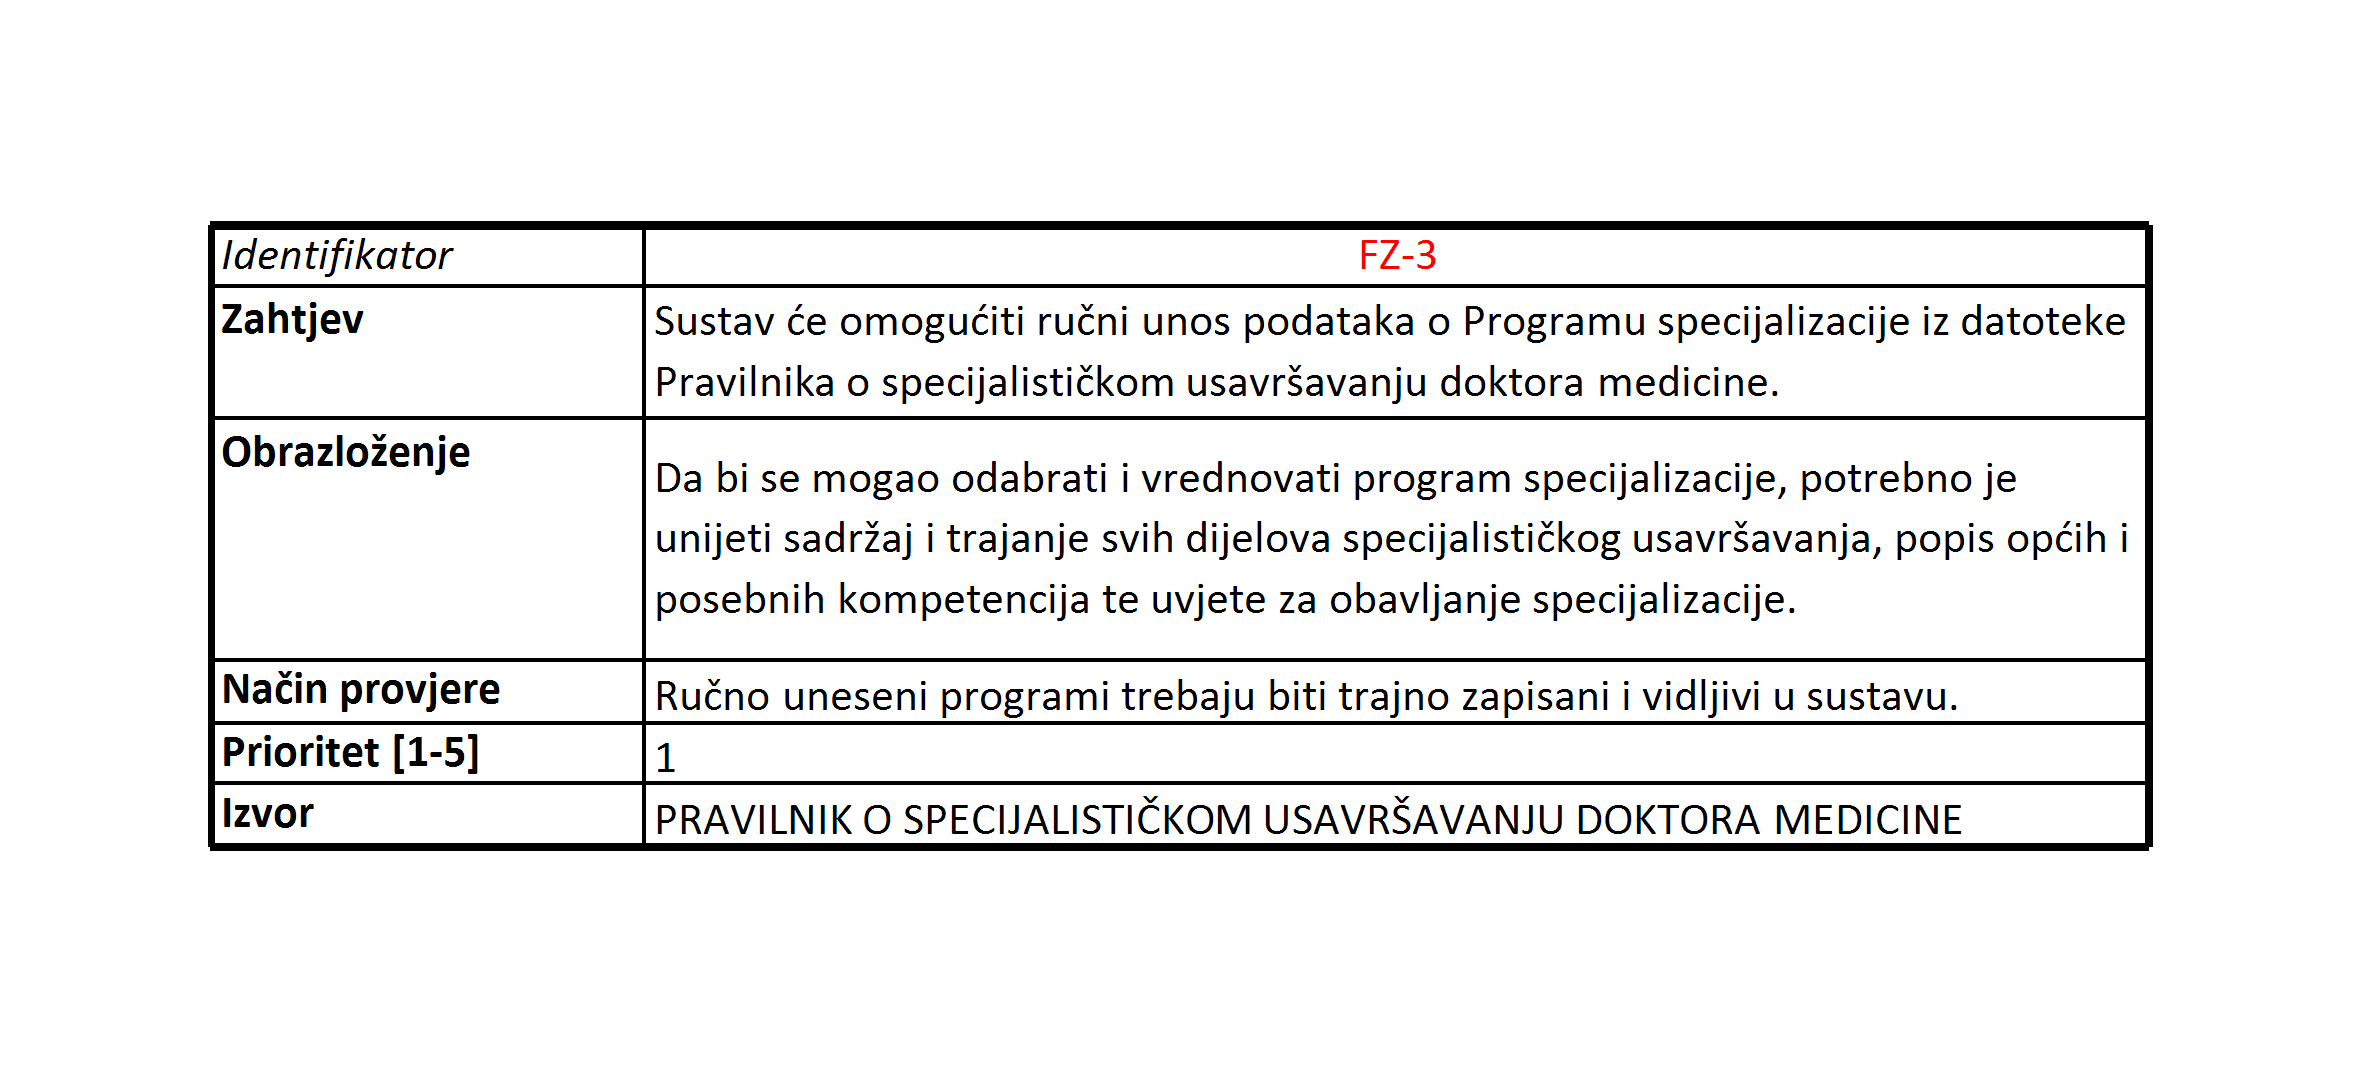
\includegraphics[width=1\textwidth]{slike/3.png}
\end{figure}
\begin{figure}[h!]
    \centering
    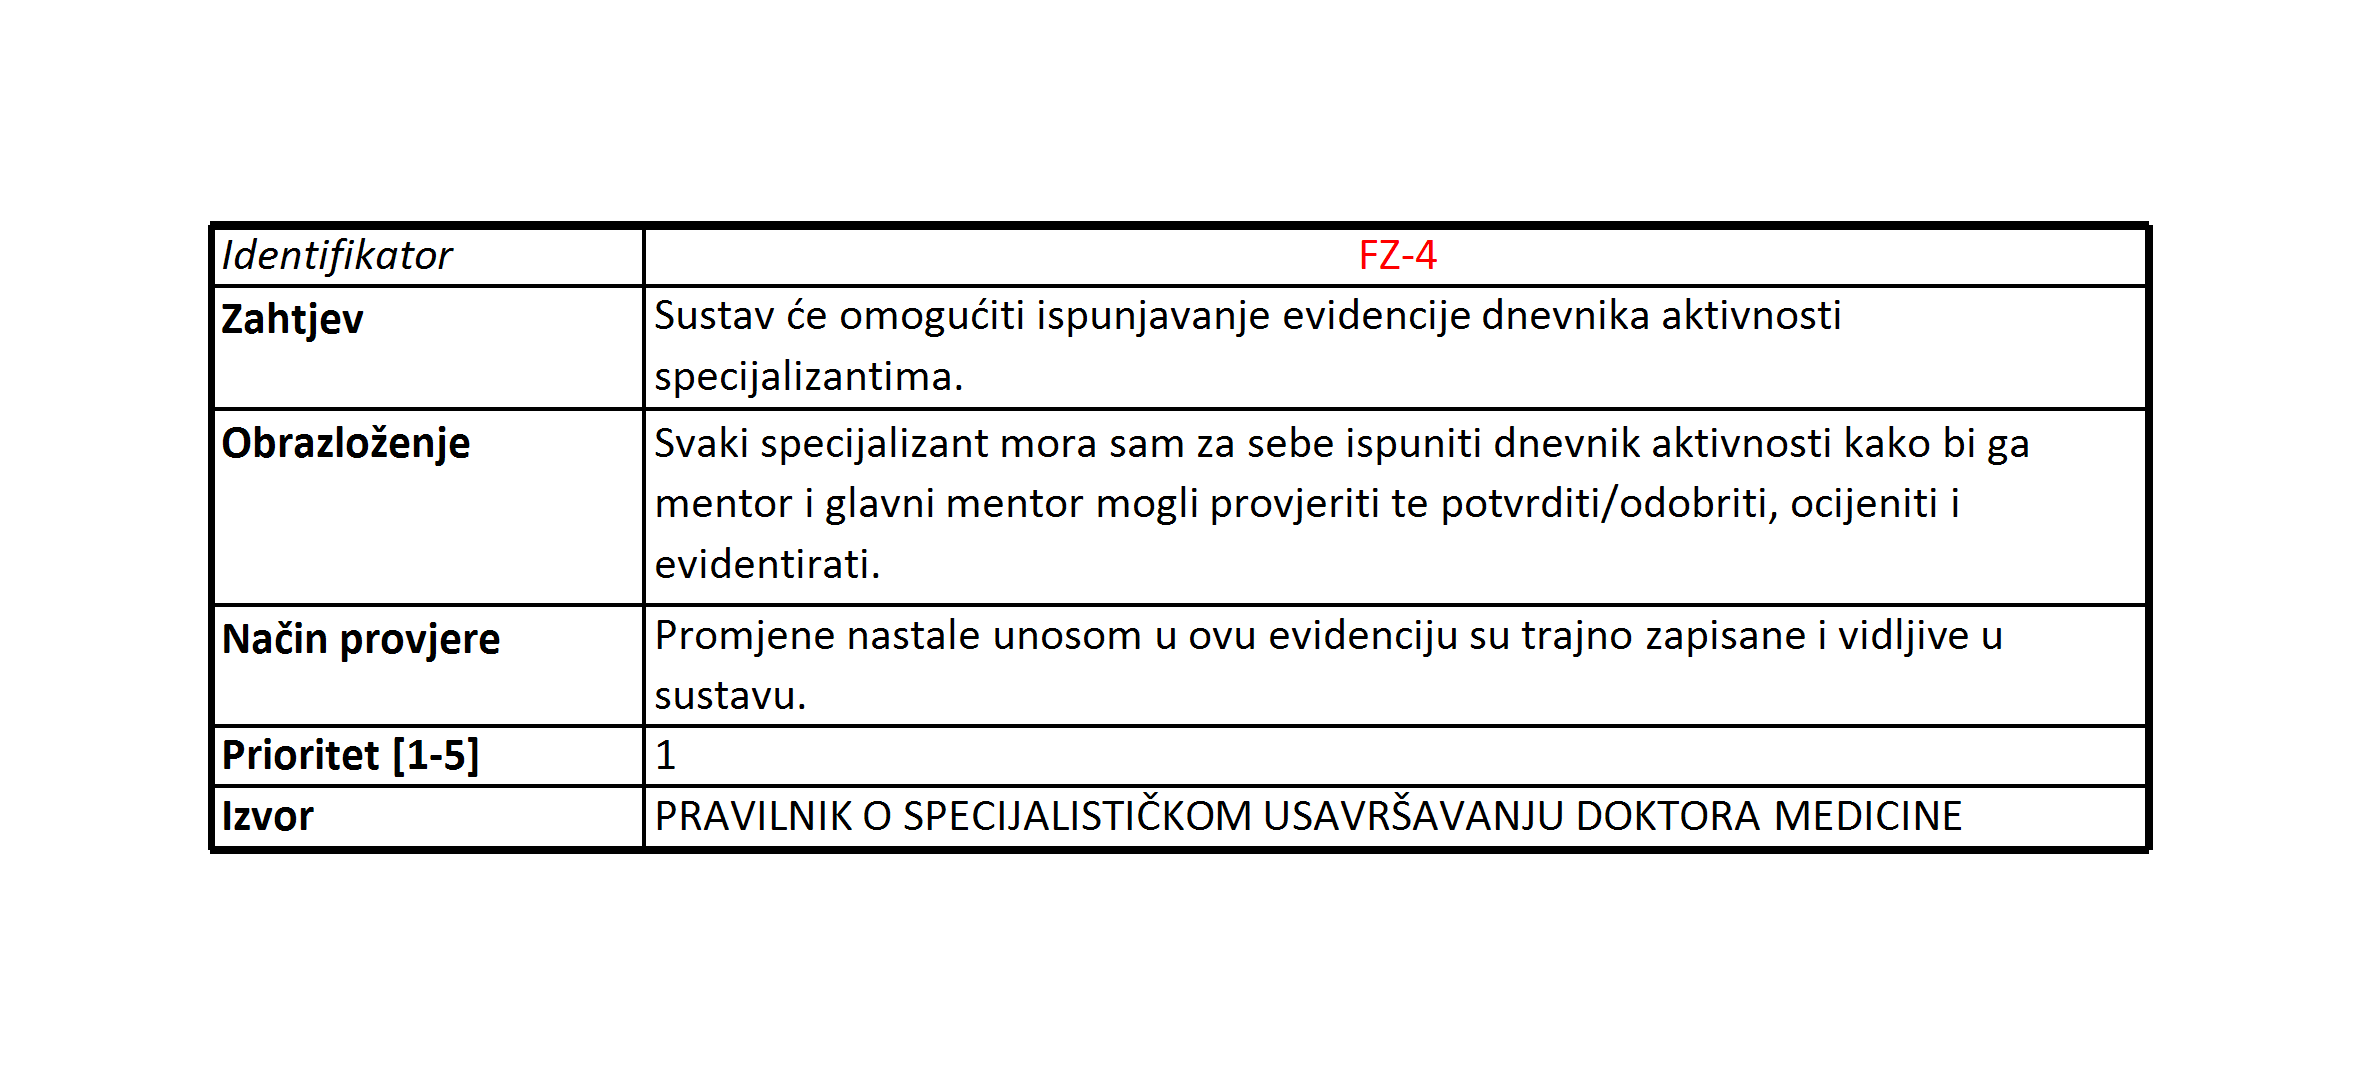
\includegraphics[width=1\textwidth]{slike/4.png}
\end{figure}
\begin{figure}[h!]
    \centering
    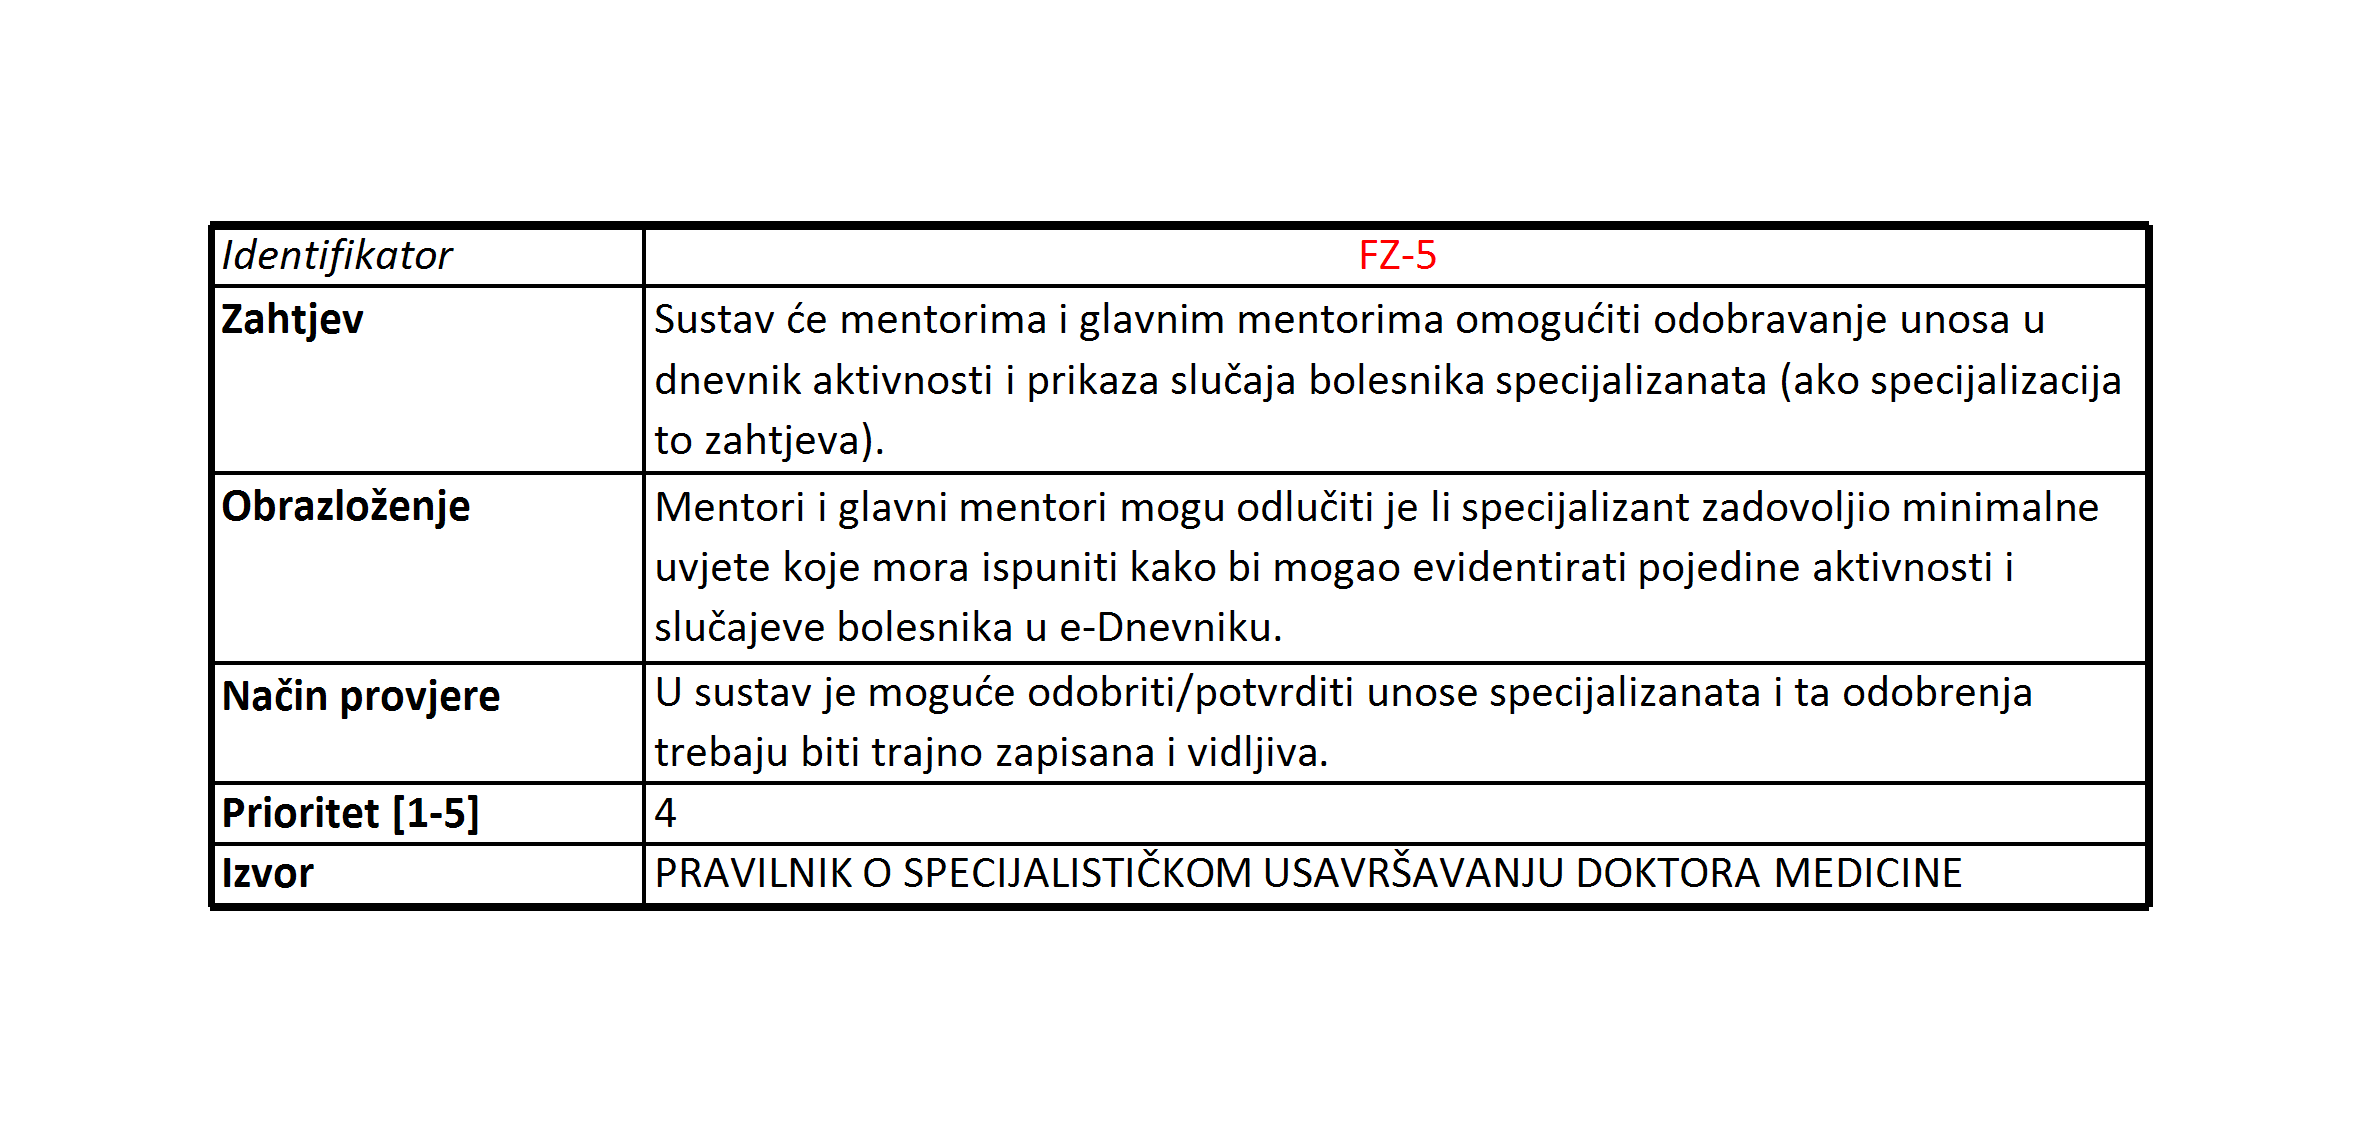
\includegraphics[width=1\textwidth]{slike/5.png}
\end{figure}
\begin{figure}[h!]
    \centering
    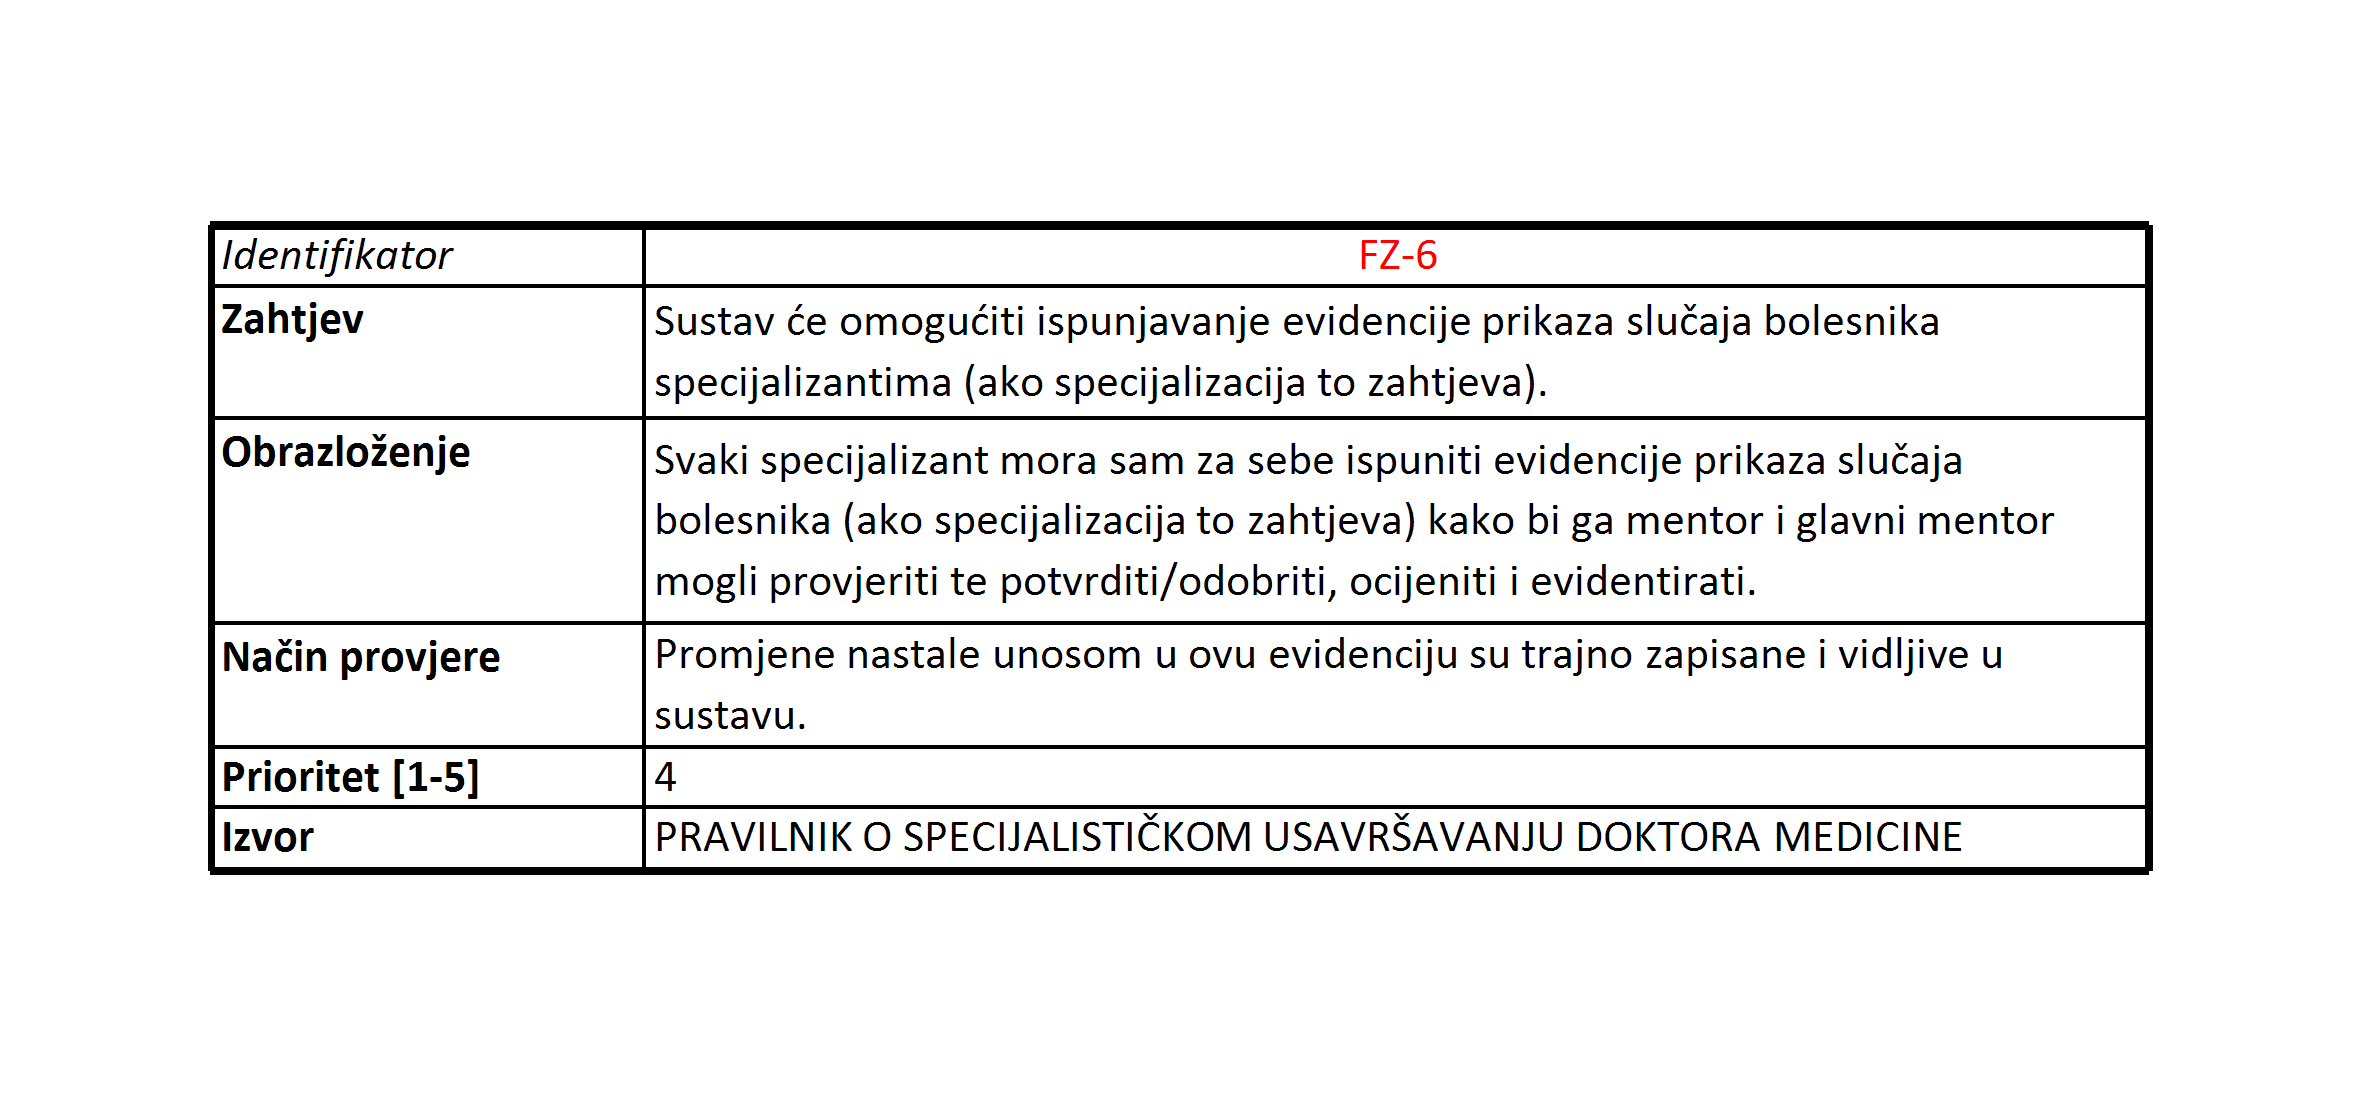
\includegraphics[width=1\textwidth]{slike/6.png}
\end{figure}
\begin{figure}[h!]
    \centering
    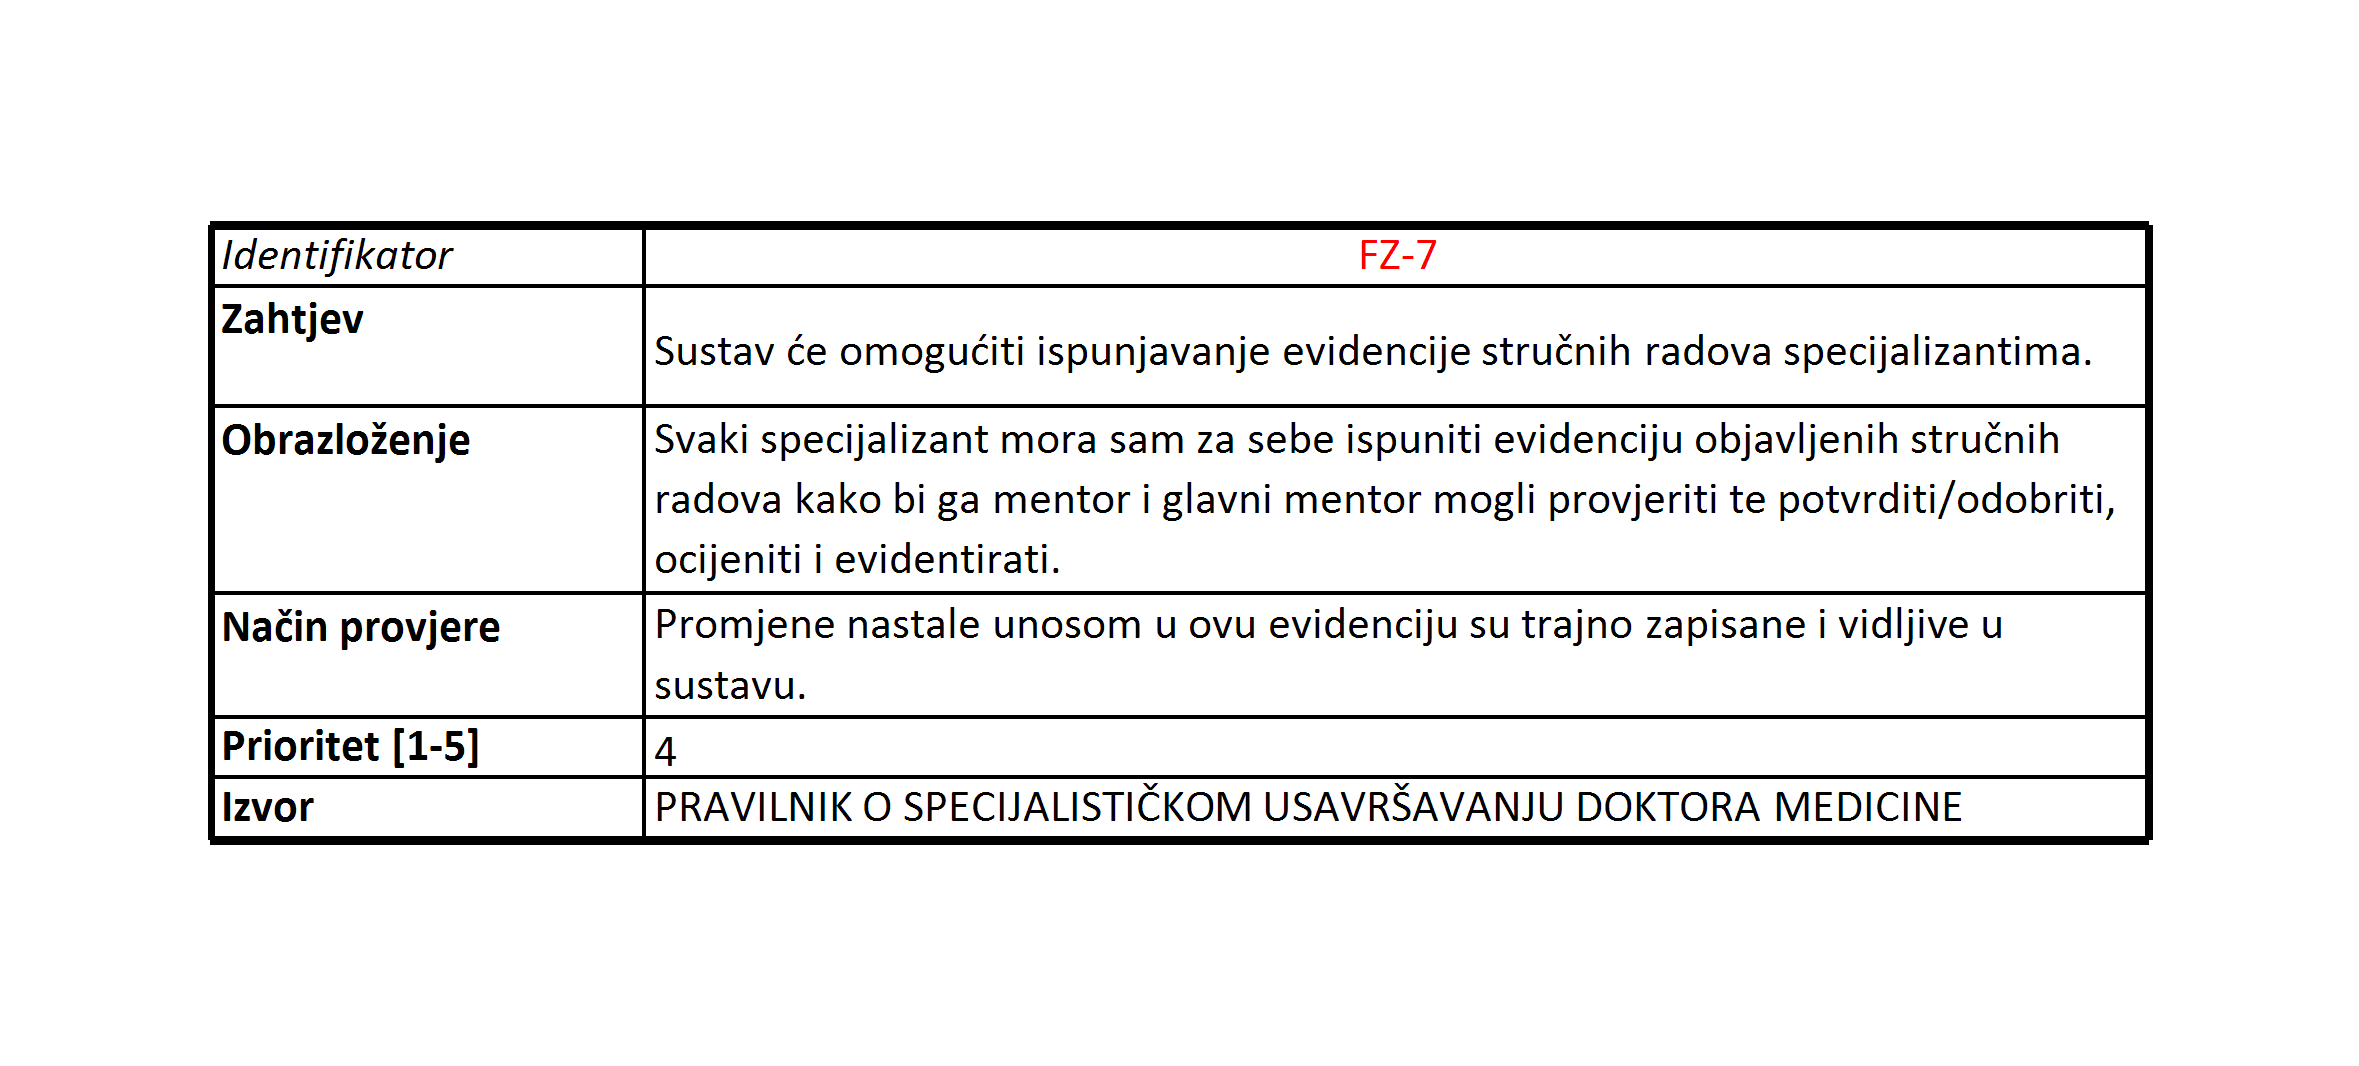
\includegraphics[width=1\textwidth]{slike/7.png}
\end{figure}
\begin{figure}[h!]
    \centering
    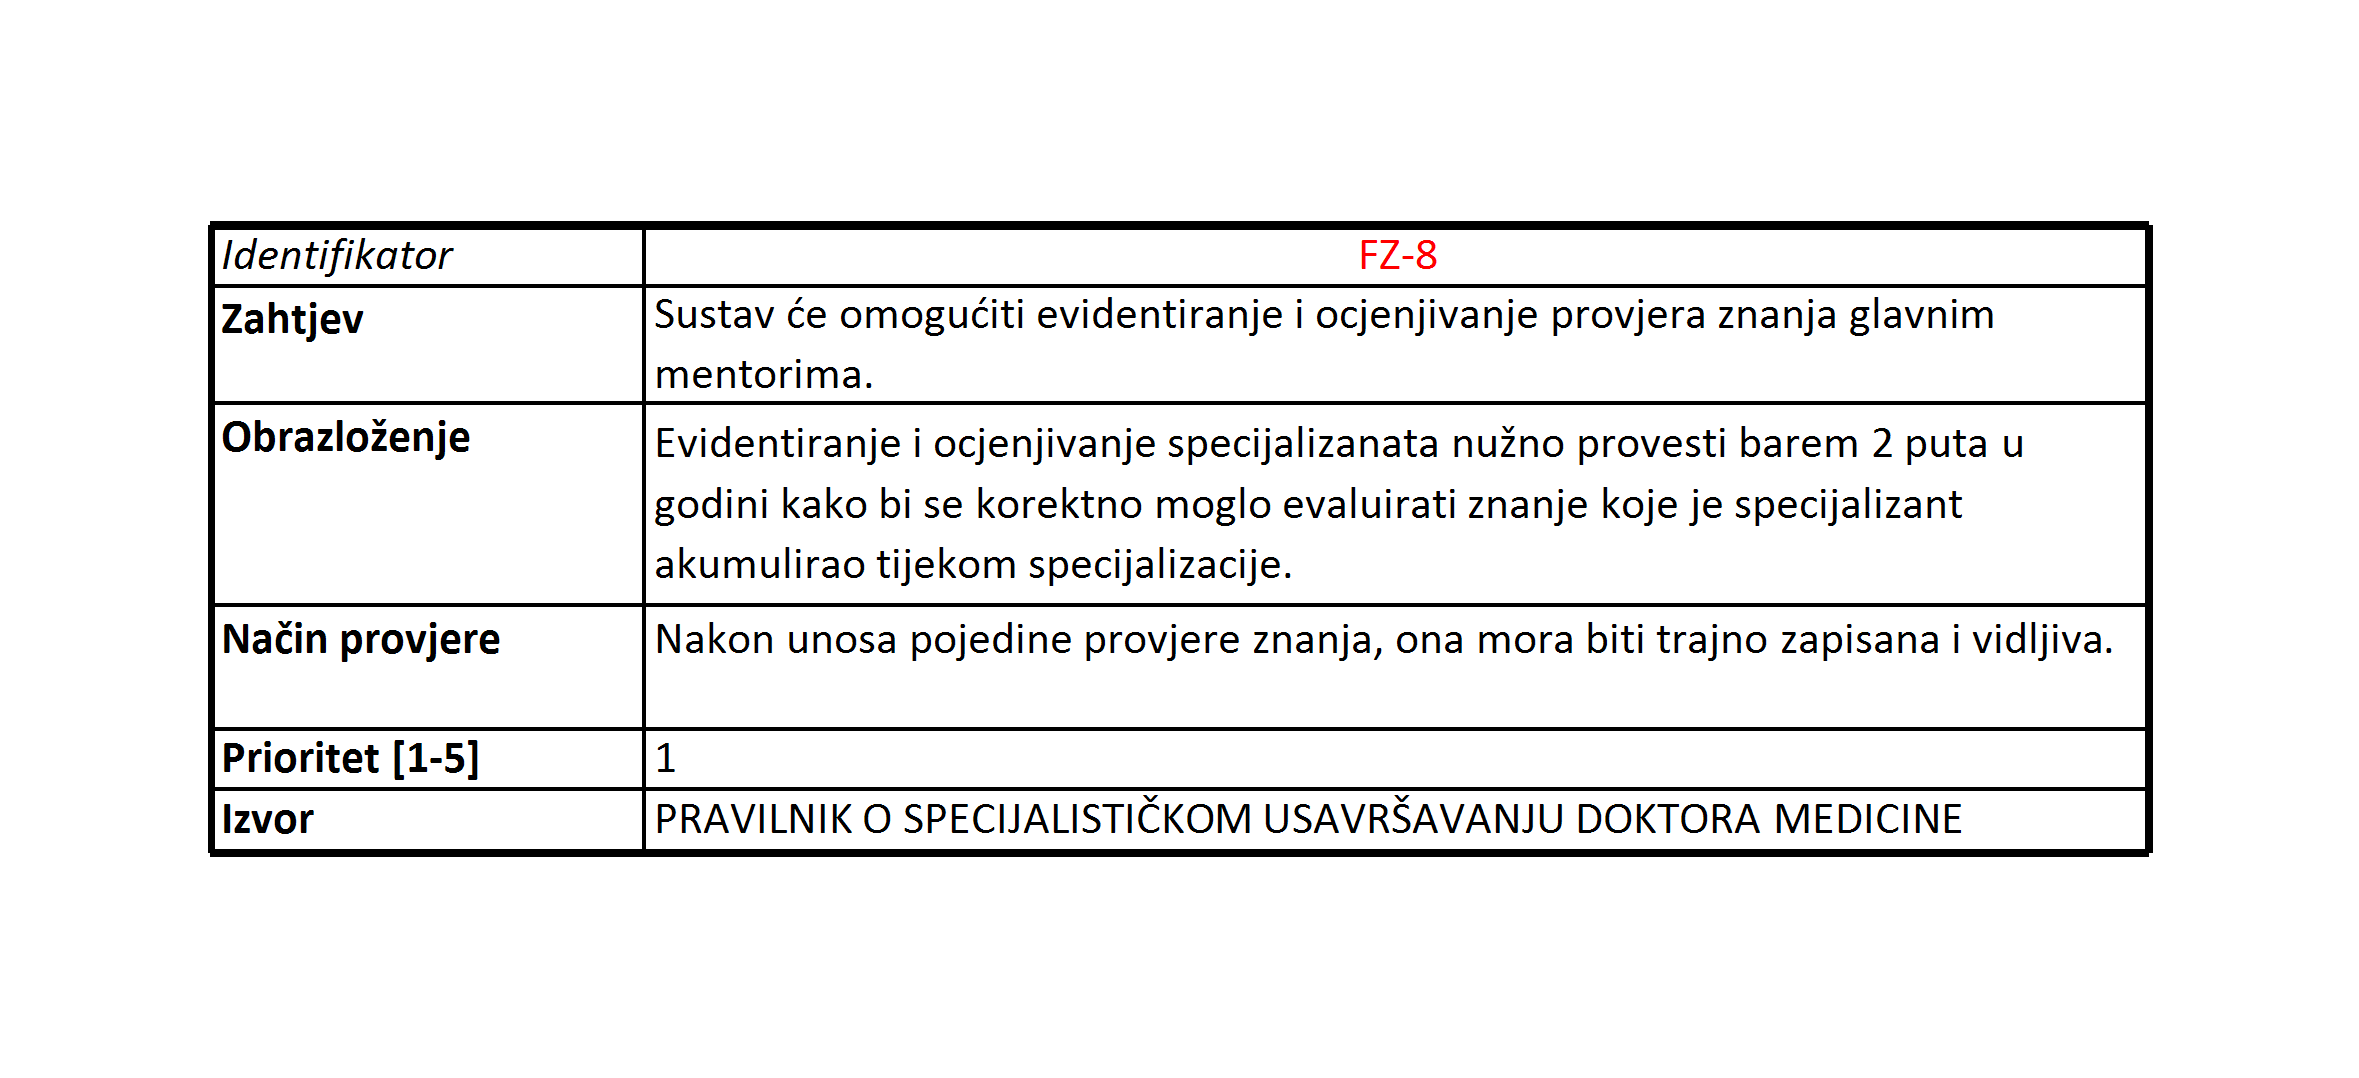
\includegraphics[width=1\textwidth]{slike/8.png}
\end{figure}
\begin{figure}[h!]
    \centering
    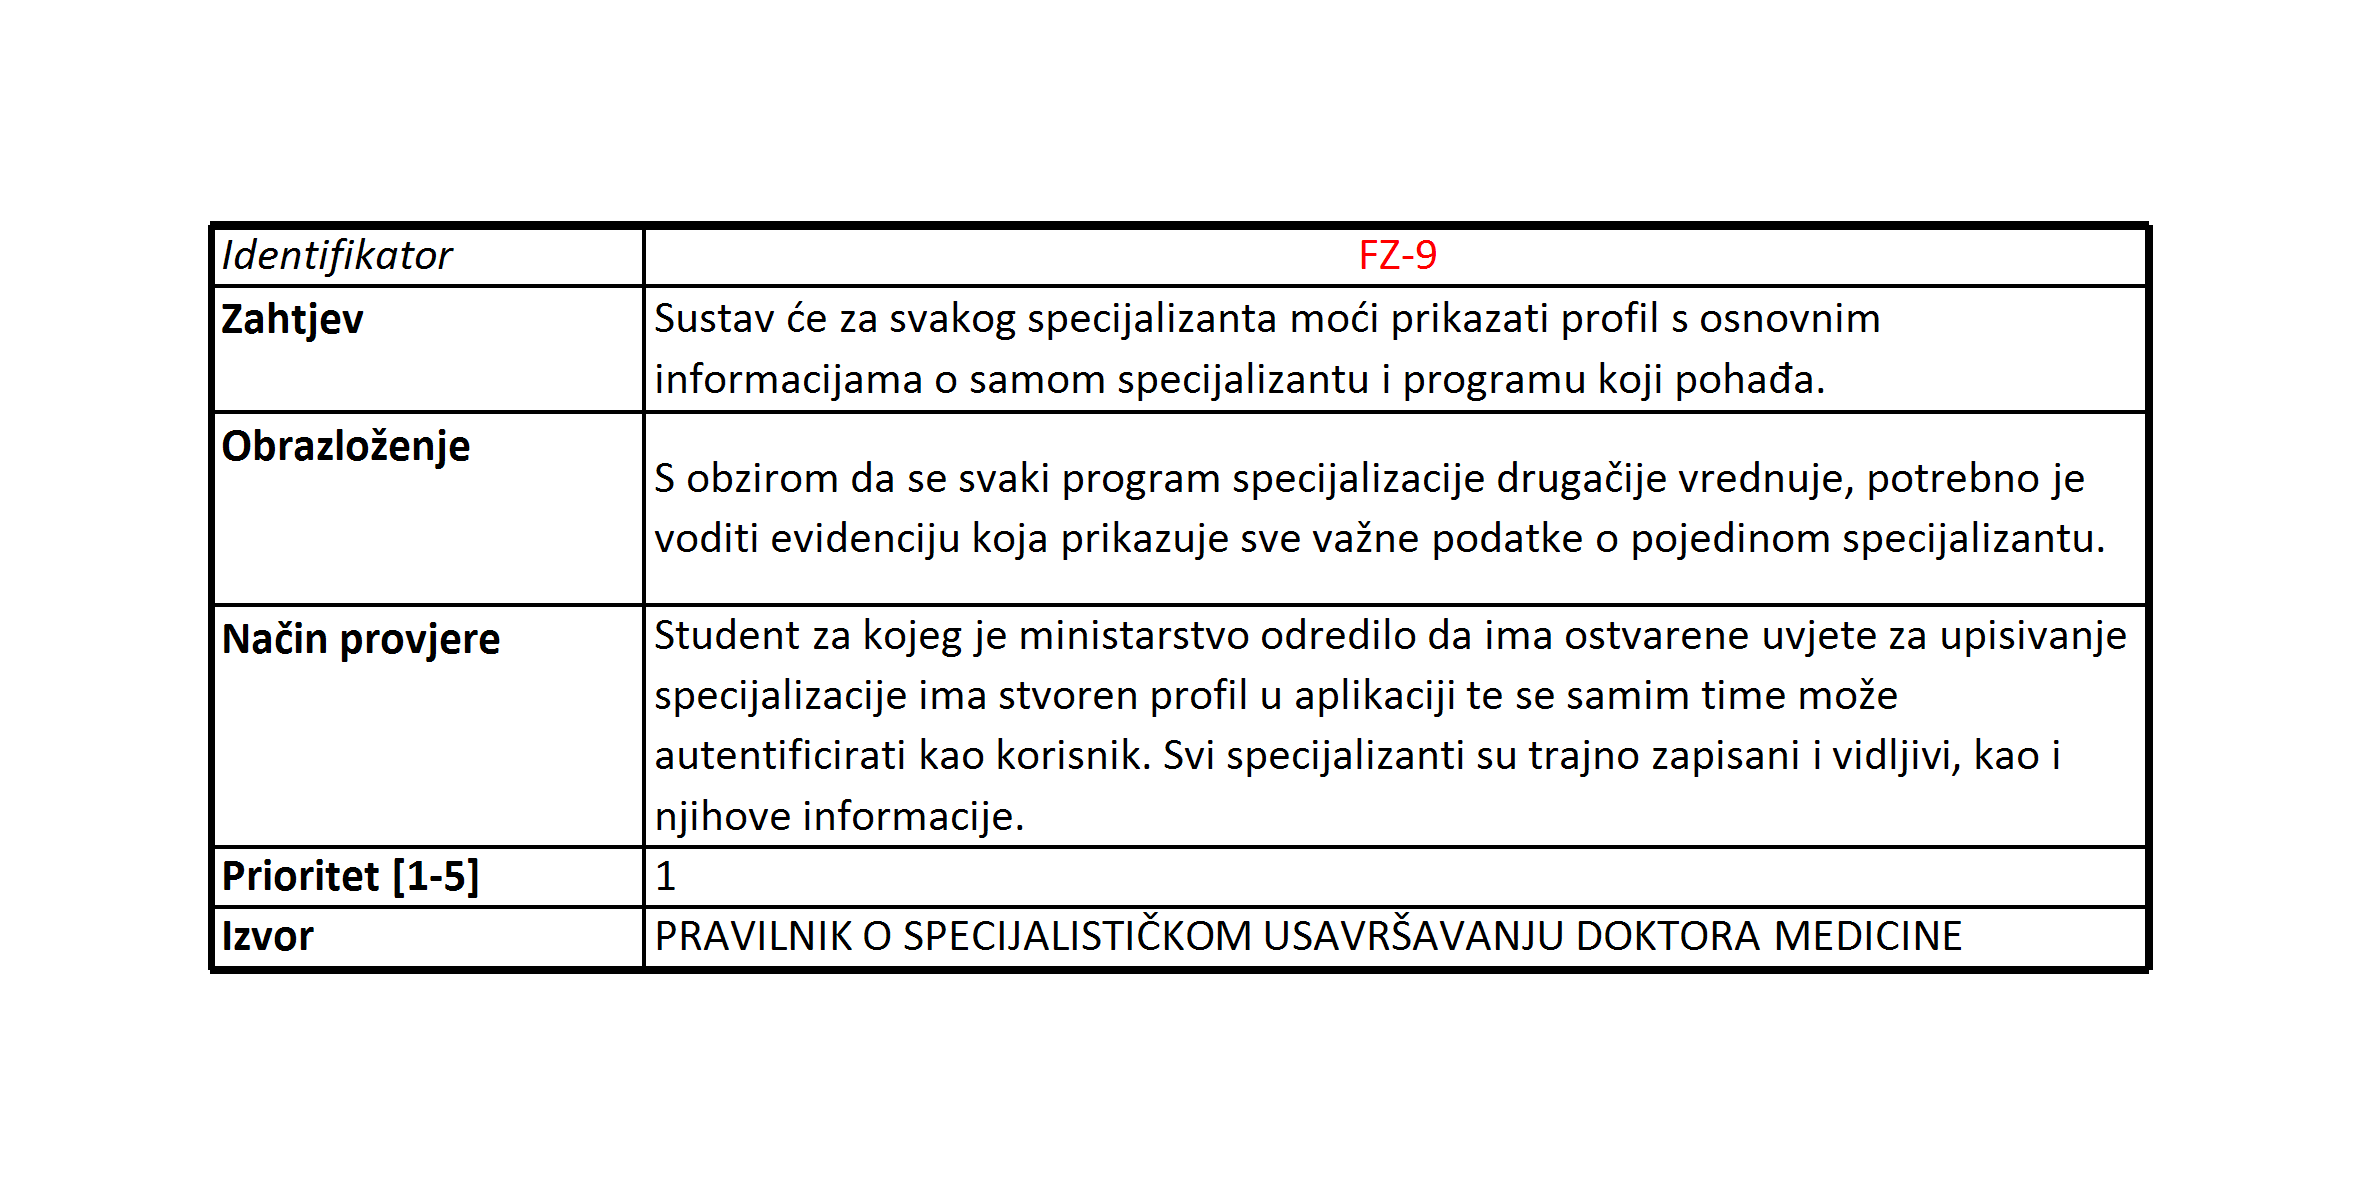
\includegraphics[width=1\textwidth]{slike/9.png}
\end{figure}
\begin{figure}[h!]
    \centering
    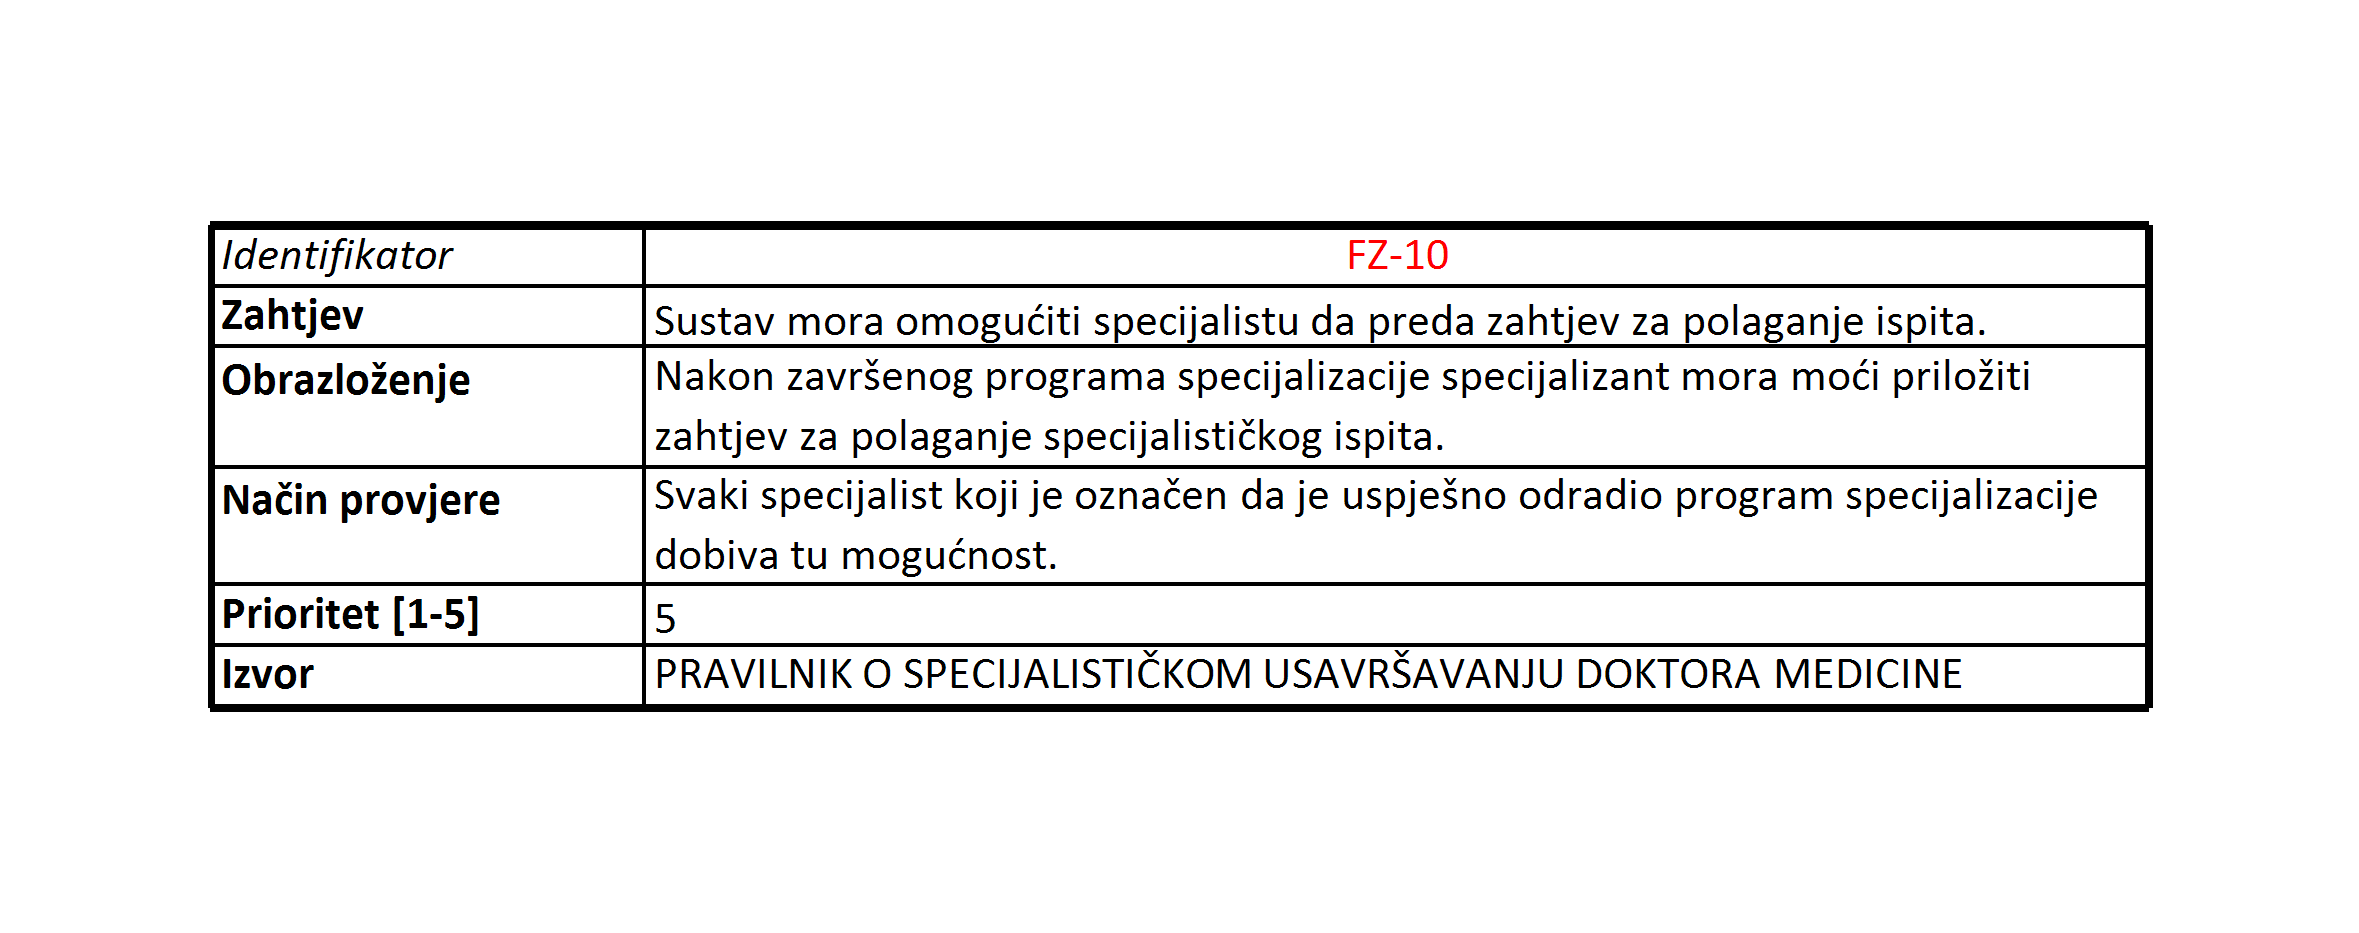
\includegraphics[width=1\textwidth]{slike/10.png}
\end{figure}
\begin{figure}[h!]
    \centering
    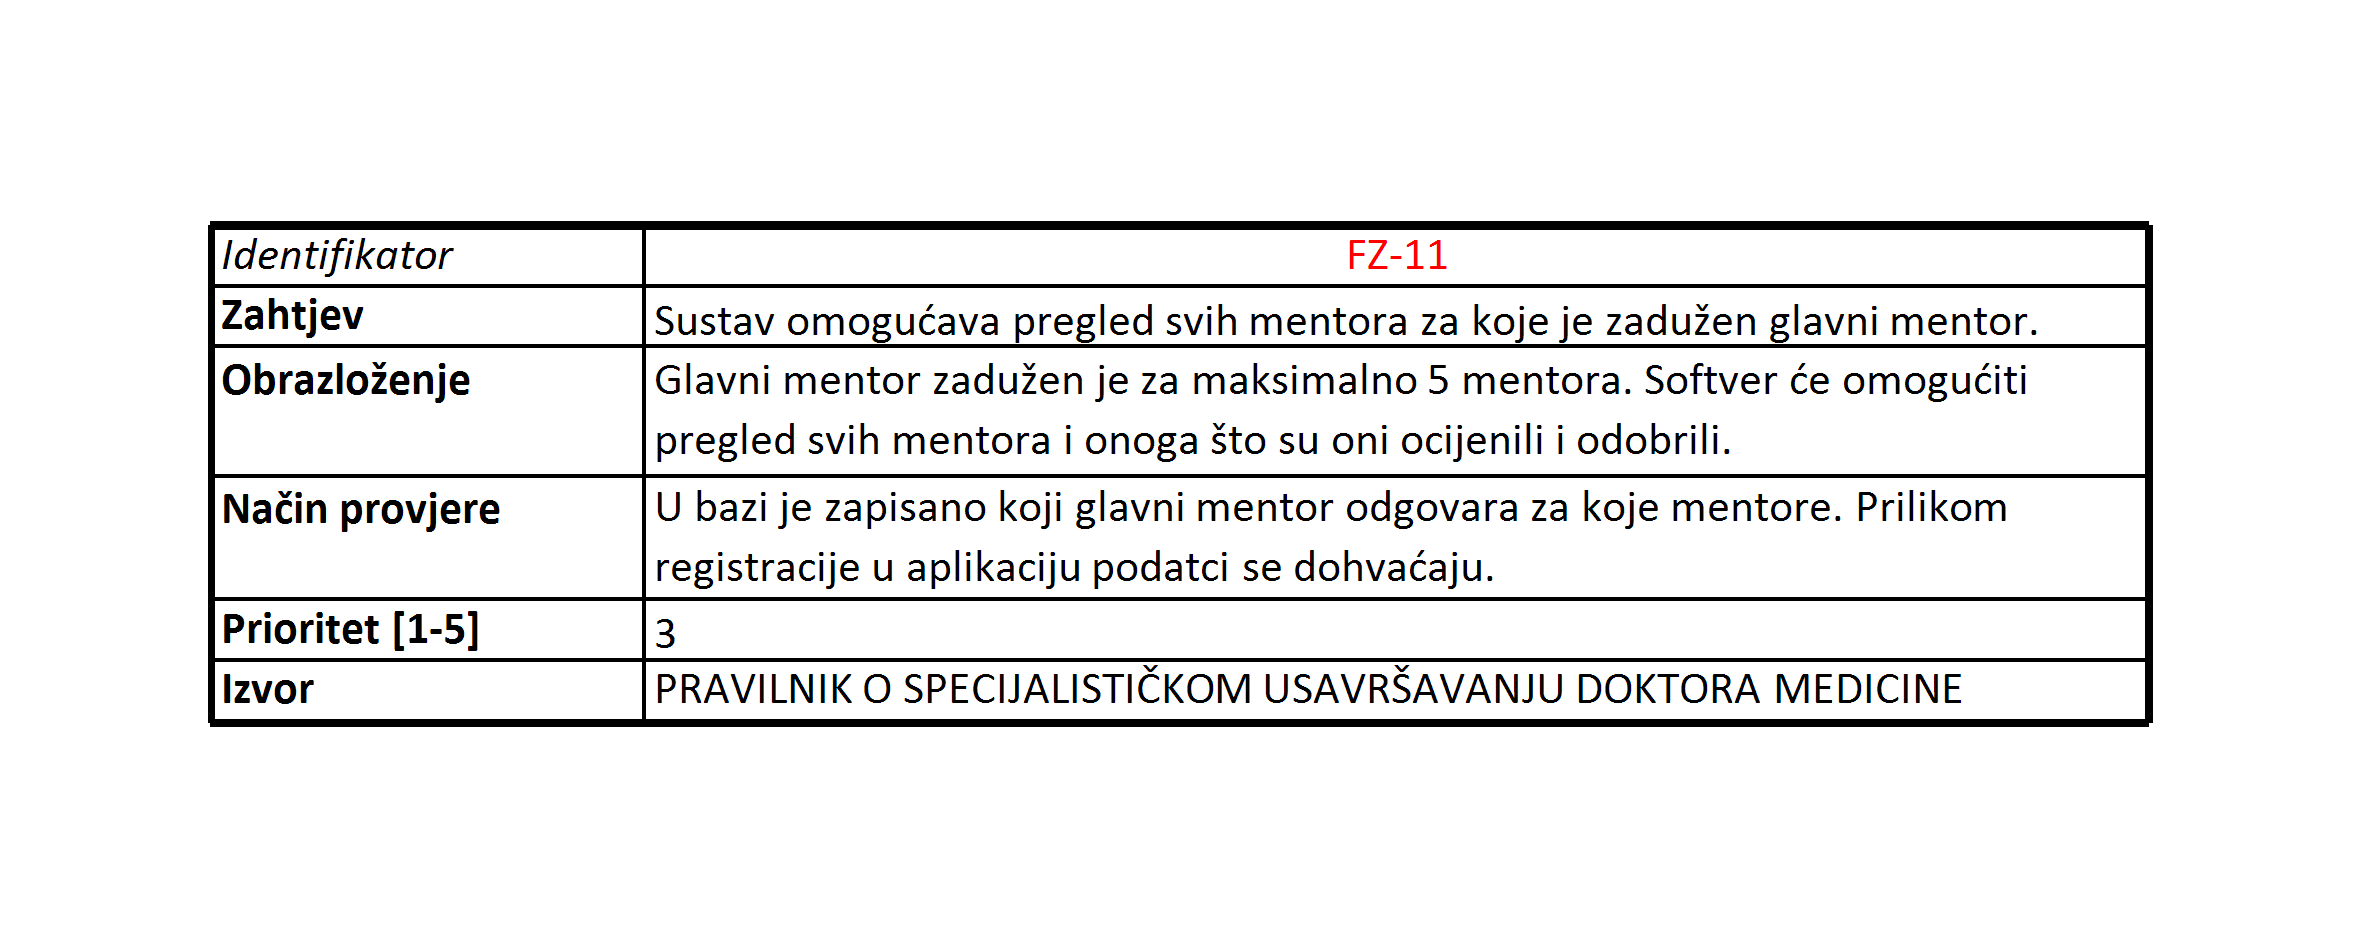
\includegraphics[width=1\textwidth]{slike/11.png}
\end{figure}
\begin{figure}[h!]
    \centering
    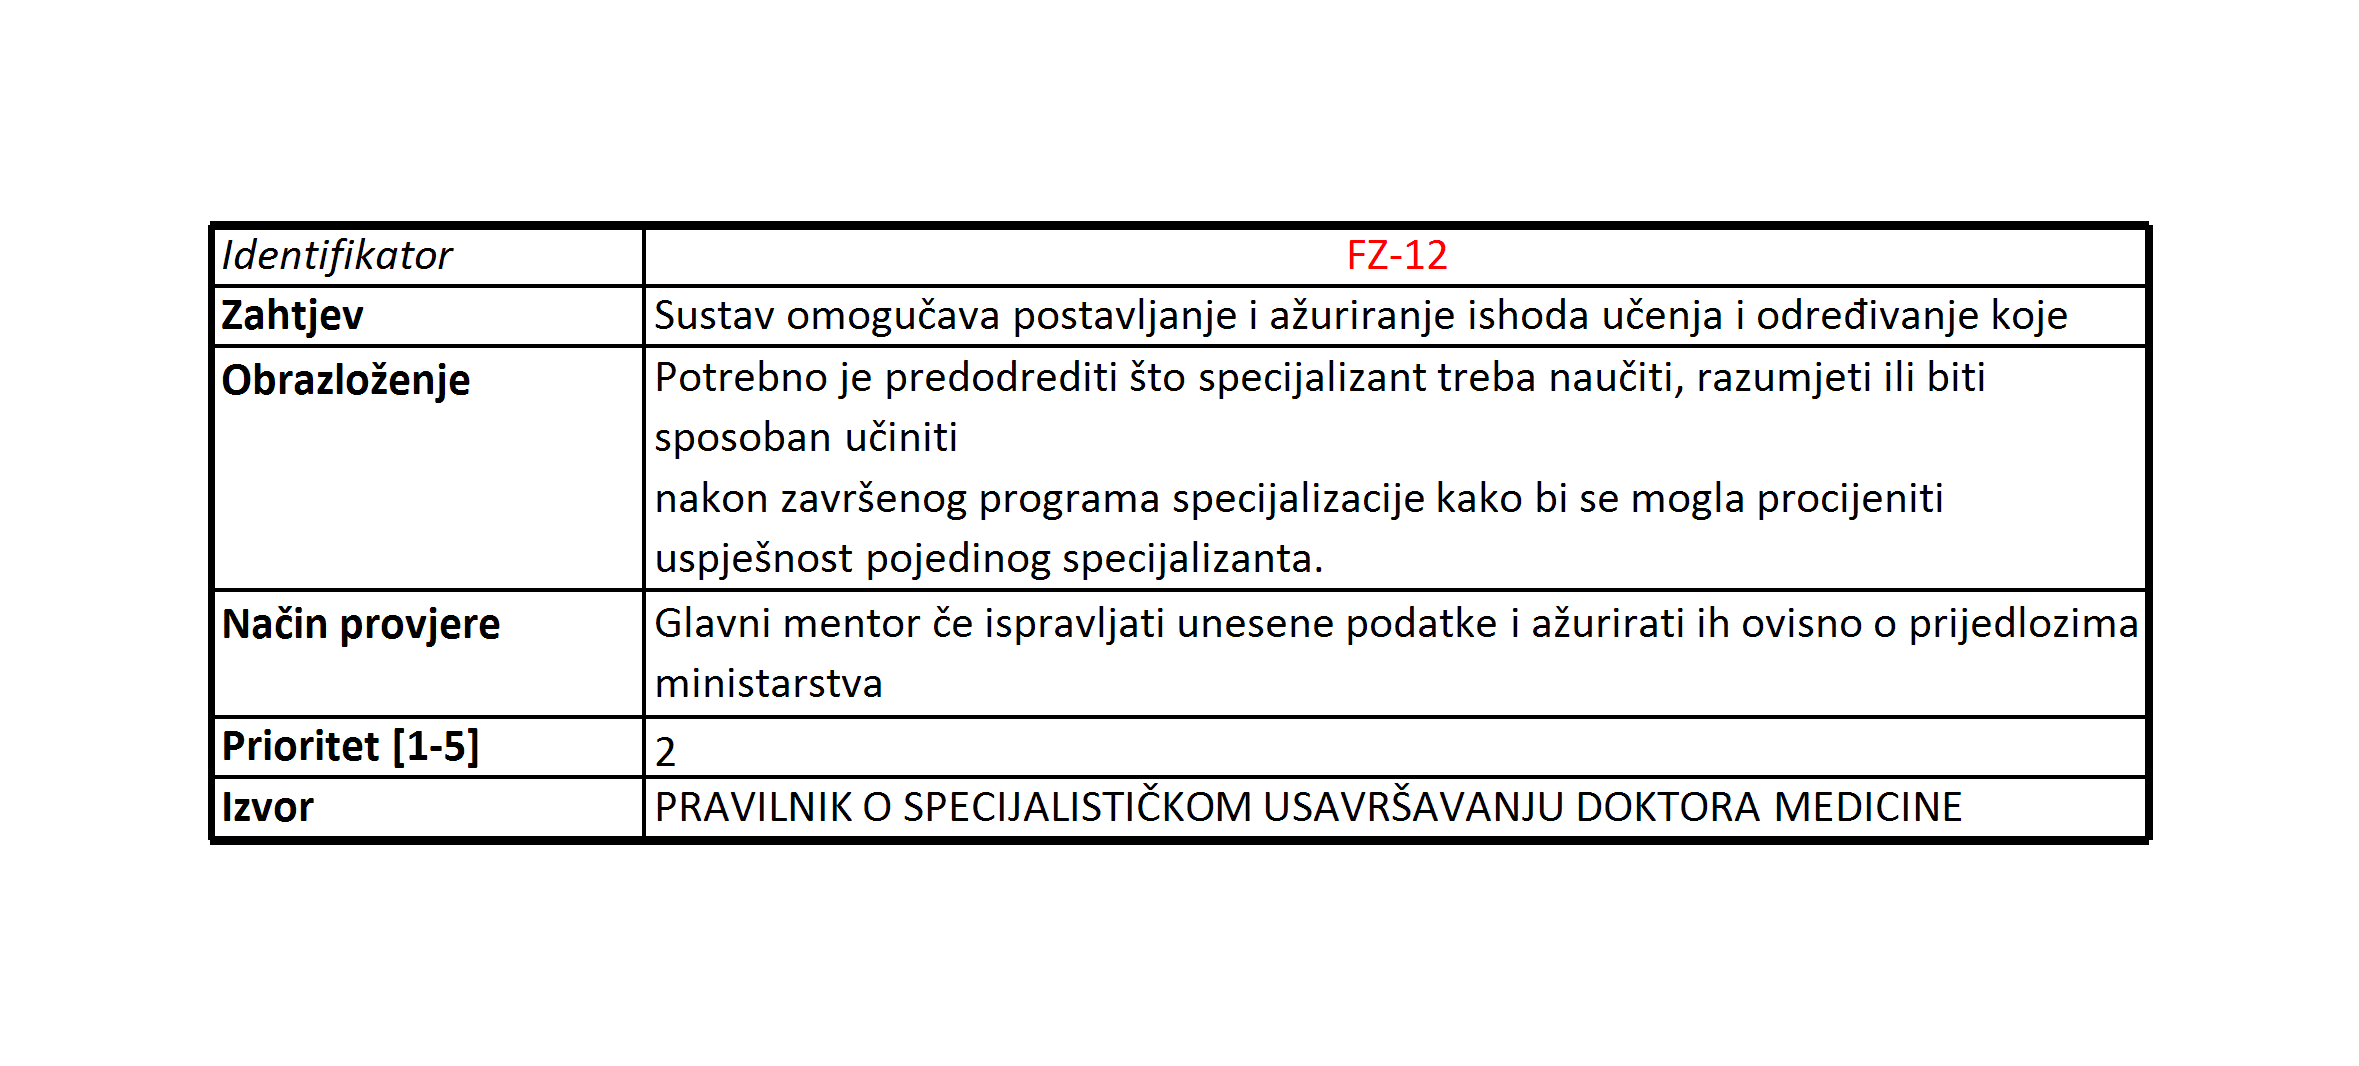
\includegraphics[width=1\textwidth]{slike/12.png}
\end{figure}

\chapter{NEFUNKCIONALNI ZAHTJEVI}

\section{Izgled softvera}
\textbf{NFZ-1} – Sustav će provoditi interakciju s korisnikom uz pomoć grafičkog sučelja.\\
\textbf{NFZ-2} – Sustav će pratiti formalan stil grafičkog sučelja.

\section{Upotrebljivost softvera}
\textbf{NFZ-3} – Sustav će ponuditi mehanizme koji će smanjiti mogućnost grešaka prilikom unosa bilo kakvih rezultata, evidencija i drugih informacija od strane definiranih korisnika.

\section{Performanse softvera}
\textbf{NFZ-4} – Sustav će osigurati preciznost za decimalne brojeve na razini 3 decimalna mjesta.\\
\textbf{NFZ-5} – Sustav će osigurati mogućnost simultanog korištenja minimalno 4 korisnika.\\
\textbf{NFZ-6} – Sustav će pokušati svesti sva kašnjenja u radu aplikacije na minimum.\\
\textbf{NFZ-7} – Sustav će biti dostupan 24 sata na dan 365 dana u godini. 

\section{Izvođenje softvera i okruženje}
\textbf{NFZ-8} – Sustav će raditi na računalima s instaliranim Windows 10 ili novijim operacijskim sustavom.

\section{Sigurnost i privatnost}
\textbf{NFZ-9} – Sustav će samo mentorima i glavnim mentorima omogućiti pristup rezultatima praćenja specijalizanta.\\
\textbf{NFZ-10} – Sustav će upotrebljavati podatke o korisnicima sukladno odredbama GDPR-a te važećim zakonima i direktivama Republike Hrvatske i Europske unije.\\
\textbf{NFZ-11} – Sustav će djelovati te propisno kazniti korisnički račun s kojeg se uoči izvođenje sumnjivih radnji.

\section{Ostalo}
Nema identificiranih dodatnih nefunkcionalnih zahtjeva.

\end{document}
